% The document class supplies options to control rendering of some standard
% features in the result.  The goal is for uniform style, so some attention 
% to detail is *vital* with all fields.  Each field (i.e., text inside the
% curly braces below, so the MEng text inside {MEng} for instance) should 
% take into account the following:
%
% - author name       should be formatted as "FirstName LastName"
%   (not "Initial LastName" for example),
% - supervisor name   should be formatted as "Title FirstName LastName"
%   (where Title is "Dr." or "Prof." for example),
% - degree programme  should be "BSc", "MEng", "MSci", "MSc" or "PhD",
% - dissertation title should be correctly capitalised (plus you can have
%   an optional sub-title if appropriate, or leave this field blank),
% - dissertation type should be formatted as one of the following:
%   * for the MEng degree programme either "enterprise" or "research" to
%     reflect the stream,
%   * for the MSc  degree programme "$X/Y/Z$" for a project deemed to be
%     X%, Y% and Z% of type I, II and III.
% - year              should be formatted as a 4-digit year of submission
%   (so 2014 rather than the accademic year, say 2013/14 say).

\documentclass[ % the name of the author
                    author={Tom Jager},
                % the name of the supervisor
                supervisor={Dr. Daniel Schien},
                % the degree programme
                    degree={MEng},
                % the dissertation    title (which cannot be blank)
                     title={A Bayesian Inference Engine for UMIS Structured Data},
                % the dissertation subtitle (which can    be blank)
                  subtitle={},
                % the dissertation     type
                      type={research},
                % the year of submission
                      year={2019} ]{dissertation}

\begin{document}

% =============================================================================

% This section simply introduces the structural guidelines.  It can clearly
% be deleted (or commented out) if you use the file as a template for your
% own dissertation: everything following it is in the correct order to use 
% as is.

% =============================================================================

% This macro creates the standard UoB title page by using information drawn
% from the document class (meaning it is vital you select the correct degree 
% title and so on).

\maketitle

% After the title page (which is a special case in that it is not numbered)
% comes the front matter or preliminaries; this macro signals the start of
% such content, meaning the pages are numbered with Roman numerals.

\frontmatter

% This macro creates the standard UoB declaration; on the printed hard-copy,
% this must be physically signed by the author in the space indicated.

\makedecl

% LaTeX automatically generates a table of contents, plus associated lists 
% of figures, tables and algorithms.  The former is a compulsory part of the
% dissertation, but if you do not require the latter they can be suppressed
% by simply commenting out the associated macro.

\tableofcontents
% \listoffigures
% \listoftables
% \listofalgorithms
% \lstlistoflistings

% The following sections are part of the front matter, but are not generated
% automatically by LaTeX; the use of \chapter* means they are not numbered.

% -----------------------------------------------------------------------------

\chapter*{Executive Summary}

{\bf A compulsory section, of at most $1$ page} 
\vspace{1cm} 

\noindent
\begin{comment}
This section should pr\'{e}cis the project context, aims and objectives,
and main contributions (e.g., deliverables) and achievements; the same 
section may be called an abstract elsewhere.  The goal is to ensure the 
reader is clear about what the topic is, what you have done within this 
topic, {\em and} what your view of the outcome is.

The former aspects should be guided by your specification: essentially 
this section is a (very) short version of what is typically the first 
chapter.  Note that for research-type projects, this {\bf must} include 
a clear research hypothesis.  This will obviously differ significantly
for each project, but an example might be as follows:

\begin{quote}
My research hypothesis is that a suitable genetic algorithm will yield
more accurate results (when applied to the standard ACME data set) than 
the algorithm proposed by Jones and Smith, while also executing in less
time.
\end{quote}

\noindent
The latter aspects should (ideally) be presented as a concise, factual 
bullet point list.  Again the points will differ for each project, but 
an might be as follows:

\begin{quote}
\noindent
\begin{itemize}
\item I spent $120$ hours collecting material on and learning about the 
      Java garbage-collection sub-system. 
\item I wrote a total of $5000$ lines of source code, comprising a Linux 
      device driver for a robot (in C) and a GUI (in Java) that is 
      used to control it.
\item I designed a new algorithm for computing the non-linear mapping 
      from A-space to B-space using a genetic algorithm, see page $17$.
\item I implemented a version of the algorithm proposed by Jones and 
      Smith in [6], see page $12$, corrected a mistake in it, and 
      compared the results with several alternatives.
\end{itemize}
\end{quote}
 
\end{comment}


\chapter*{Supporting Technologies}

\begin{comment}
{\bf A compulsory section, of at most $1$ page}
\vspace{1cm} 

\noindent
This section should present a detailed summary, in bullet point form, 
of any third-party resources (e.g., hardware and software components) 
used during the project.  Use of such resources is always perfectly 
acceptable: the goal of this section is simply to be clear about how
and where they are used, so that a clear assessment of your work can
result.  The content can focus on the project topic itself (rather,
for example, than including ``I used \mbox{\LaTeX} to prepare my 
dissertation''); an example is as follows:

\begin{quote}
\noindent
\begin{itemize}
\item I used the Java {\tt BigInteger} class to support my implementation 
      of RSA.
\item I used a parts of the OpenCV computer vision library to capture 
      images from a camera, and for various standard operations (e.g., 
      threshold, edge detection).
\item I used an FPGA device supplied by the Department, and altered it 
      to support an open-source UART core obtained from 
      \url{http://opencores.org/}.
\item The web-interface component of my system was implemented by 
      extending the open-source WordPress software available from
      \url{http://wordpress.org/}.
\end{itemize}
\end{quote}
 
 
- Python
- Pymc3
- Theano
- Seaborn
- Pandas
\end{comment}

% -----------------------------------------------------------------------------

\chapter*{Notation and Acronyms}

{\bf An optional section, of roughly $1$ or $2$ pages}
\vspace{1cm} 

\noindent
Any well written document will introduce notation and acronyms before
their use, {\em even if} they are standard in some way: this ensures 
any reader can understand the resulting self-contained content.  

Said introduction can exist within the dissertation itself, wherever 
that is appropriate.  For an acronym, this is typically achieved at 
the first point of use via ``Advanced Encryption Standard (AES)'' or 
similar, noting the capitalisation of relevant letters.  However, it 
can be useful to include an additional, dedicated list at the start 
of the dissertation; the advantage of doing so is that you cannot 
mistakenly use an acronym before defining it.  A limited example is 
as follows:

\begin{quote}
\noindent
\begin{tabular}{lcl}
CC                 &:     & Concentration Coefficient
  \\
ERN                &:     & Entity Relationship Diagram
   \\
IE                 &:     & Industrial Ecology                                         \\
IOA                &:     & Input Output Assessment
  \\
LCA                &:     & Life Cycle Assessment
  \\
MC             &:      &  Monte Carlo
  \\
MCMC             &:      &  Markov Chain Monte Carlo
  \\
MFA                &:     & Material Flow Assessment
  \\
pdf             &:       & Probability density function
 \\
STAF               &:     & Stocks and Flows
 \\
STAFDB             &:      &  Stocks and Flows Database
  \\
TC                 &:     & Transfer Coefficient
 \\
UMIS               &:     & Unified Materials Information System
  \\
YSTAFDB            &:     & Yale Stocks and Flows Database
  \\

\end{tabular}
\end{quote}

% -----------------------------------------------------------------------------

\chapter*{Acknowledgements}
\begin{comment}
{\bf An optional section, of at most $1$ page}
\vspace{1cm} 

\noindent
It is common practice (although totally optional) to acknowledge any
third-party advice, contribution or influence you have found useful
during your work.  Examples include support from friends or family, 
the input of your Supervisor and/or Advisor, external organisations 
or persons who  have supplied resources of some kind (e.g., funding, 
advice or time), and so on.
 
\end{comment}

% =============================================================================

% After the front matter comes a number of chapters; under each chapter,
% sections, subsections and even subsubsections are permissible.  The
% pages in this part are numbered with Arabic numerals.  Note that:
%
% - A reference point can be marked using \label{XXX}, and then later
%   referred to via \ref{XXX}; for example Chapter\ref{chap:context}.
% - The chapters are presented here in one file; this can become hard
%   to manage.  An alternative is to save the content in seprate files
%   the use \input{XXX} to import it, which acts like the #include
%   directive in C.

\mainmatter

% -----------------------------------------------------------------------------

\chapter{Contextual Background}
\label{chap:context}

\noindent
\section{Industrial Ecology}

Industrial ecology (IE) is an area of research focused around the flow of material, energy and money through a system. It can also be described as socio-economic metabolism (SEM) as it models the production, consumption and storage of resources by society. It primarily focuses on the relationship between human originating sectors (anthroposphere) and the natural ecosystem by modelling industrial infrastructures as their own subsystems that interact with their environment \cite{tibbs1992industrial}. The International Society for Industrial Ecology uses the following definition by White, "the study of the flows of materials and energy in industrial and consumer activities, of the effects of these flows on the environment, and of the influences of economic, political, regulatory and social factors on the flow, use and transformation of resources" \cite{white1994greening}. As such it is a multi-disciplinary field which seeks to account for material and energy data and use it to inform social and economic policy as well as business strategy. The primary motivator for Industrial Ecology is to encourage and ensure sustainable development. By most agreed definitions, this involves ensuring that the economical and societal growth occurs without hampering the ability of development in the future \cite{robert2005sustainable}. Therefore research in Industrial Ecology focuses on decoupling the relationship industrial development has on natural ecosystems. To do this, the entire life cycle of products and materials are analyzed in order to find areas for greater efficiency and reduced reliance on natural resources. Studies in Industrial Ecology can focus on identifying the amount of flow of specific materials from the anthroposphere into the environment \cite{rockstrom2009safe}, to assessing where new stocks of materials are accumulating \cite{müller2014modeling}, or finding energy and material "loops" which can be closed in order to reuse waste material and energy\cite{esty1998industrial}.

\subsection{Industrial Ecology Methodology}
There exist a variety of different methodologies to conduct studies in Industrial Ecology. The data resulting from IE studies therefore is usually in a format only suited for that methodology. The three most prevalent methods are Life Cycle Assessments (LCAs), Input-Output Analysis (IOA) and Material Flow Analysis (MFA) \cite{myers2019unified}.

Life Cycle Assessments follow the environmental impact of a product system throughout its life cycle \cite{ISO14040}. It often involves compiling an inventory analysis where the life cycle is modelled as a system of processes with material and energy flowing between them. Inputs and outputs from each process are specified with special interest paid to flows into and from the environment. This is used to assess the impact of a product and provide information for corporate decision making in order to improve the efficiency of a product. Other motivators are in reducing a product's environmental impact. LCAs have been known to have sector wide impacts through industry collaboration \cite{mattila2012methodological}. Open data formats such as EcoSpold and ILCD as well as shared databases such as Ecoinvent \cite{wernet2016ecoinvent}, make this possible as different industry partners can combine research and also easily recreate results to ensure accuracy. 

Input-Output Analyses takes an economic approach to IE and tracks the flow of money between entities in a geographic region. These can then be used to allocate environmental impact to these entities. As economic data on inter-sector flows are generally more granular than data on the movement of physical material, it can be useful to apply data from IOAs in studies that use other methodologies \cite{chen2016building}.

Material and Energy Flow Analyses maps the presence of a specific material(s) in a system, paying particular attention to where it accumulates in the form of stocks. It does this by modelling a system as a collection of processes and then accounting for flows between and the build up of stocks in them. This is useful for identifying where cycles can be created and enhanced in these systems in order to increase recycling and therefore reduce a system's dependence on its environment \cite{müller2014modeling}. Static MFAs are where the scope of the analyses falls over a single specified timeframe, whilst dynamic MFAs use data about past and present quantities to estimate future impacts. This can highlight which resources may become scarce in the future and provide warnings about future environmental impacts.

\section{Unifying Industrial Ecology}
Whilst some studies have incorporated data from one methodology into another \cite{chen2016building}, there is need to provide a common framework for all varieties of industrial ecological data. In \cite{pauliuk2015general}, Pauliuk et al performed a comprehensive analysis on the myriad of methodologies present in IE. They discovered that each methodology described the system using a shared structure, that of a bipartite directed graph. The shared common property between each system is that material was \textit{transformed} in one process and then \textit{distributed} in a subsequent process. Edges in this bipartite graph denote a flow of material from one a \textit{distribution} node to a \textit{transformation} node or vice versa.

\subsection{STAFDB and UMIS}
Over the past 20 years, the Graedal research group at Yale University have compiled Industrial Ecology data on over 100 materials on a variety of spacial and temporal scales. The data from these studies has been extracted and used to create the Yale Stocks and Flows Database (YSTAFDB) \cite{ystafdb}. Ongoing work by Myers, Hoekman and Petard (to be published), is in developing a community driven database for this data called the Stocks and Flows Database (STAFDB). This is an improvement on YSTAFDB as it is designed to be more user friendly and deals with the problem of divergent disaggregation.

Disaggregation is where a property of data (e.g a process that data is coming from or the material being described) is divided into components. In a broad example, data about cars could be disaggregated into electric and non-electric vehicles or large and small cars. If data from two studies with different techniques of disaggregation (or divergent disaggregation) on the same data were structured into the same system, data could be counted twice when performing analysis \cite{myers2019unified}. To prevent this, process and material data in STAFDB contains a parent field and an \texttt{is\_separator} flag which serves to keep track of methods of disaggregation and prevent double counting.

Myers et al. has created UMIS, the Unified Materials Information System \cite{myers2019unified} as a data format to structure data contained in STAFDB. UMIS structures stocks and flows data that comprise IE studies into a format that is agnostic to IOA, MFA and LCA methodologies as a UMIS diagram. This diagram can displayed visually and is also machine readable which allows for greater automation when dealing with stocks and flows data.

UMIS is a step in shifting industrial ecology towards a more virtual platform where industrial ecological data can be stored in a centralized knowledge base, with an ecosystem of tools and routines to develop models and analyze the data for further studies. This would reduce the time taken to perform further studies, allow of greater collaboration in the field and provide greater transparency on the results of studies \cite{hertwich2018nullius}. An example of such a platform is the Metabolism Of Cities project, a digital research lab created by Paul Hoekman \cite{MetabolismOfCities}. The platform's primary aim is to encourage research and allow collaboration in studying the metabolism of resources and energy surrounding specific regions. It contains a store of publications, IE data and an online material flow analysis tool to allow users to easily conduct MFA studies and interface with a common online database. Work is currently being done to integrate metabolism of cities with STAFDB to allow for future research to be directly inserted into the database. 

\subsection{UMIS Terminology}
The components and design of a UMIS diagram are drawn from MFA concepts but can still be reconciled with IOA and LCA data. A definition list for the components of a UMIS diagram can be found in table \ref{umis_terms}.

\begin{table}[ht]
\begin{tabular}{|l|l|}
\hline
{\textbf{UMIS Component}}   & {\textbf{Definition}}                                                                                                                                                                                                                                          \\ \hline
System Boundary        & \begin{tabular}[c]{@{}l@{}}Definition of the boundary of the data. This is defined by the reference\\ space, time frame and material. Provides a limit of what parts of the real\\ world we are interested in and modelling in this system\end{tabular}   \\ \hline
Reference Space        & \begin{tabular}[c]{@{}l@{}}The geographical space within which all processes, stocks and flows\\ internal to the UMIS diagram reside.\end{tabular}                                                                                                        \\ \hline
Reference Material     & \begin{tabular}[c]{@{}l@{}}The material whose stocks and flows are described in the diagram. Can be\\ at a high level of disaggregation (e.g a diagram with a reference material\\ of Steel can contain stocks and flows of Carbon and Iron)\end{tabular} \\ \hline
Reference Time frame   & The time frame over which material is flowing or is stocked.                                                                                                                                                                                              \\ \hline
Process                & An event involving a material                                                                                                                                                                                                                             \\ \hline
Transformation Process & A process where an object is transformed into another object                                                                                                                                                                                              \\ \hline
Distribution Process   & A process where an object is transferred to another process or location                                                                                                                                                                                   \\ \hline
Storage Process        & A process where material is moved into or from storage                                                                                                                                                                                                    \\ \hline
Stock                  & Movement of material between a process and storage                                                                                                                                                                                                        \\ \hline
Flow                   & \begin{tabular}[c]{@{}l@{}}Movement of material between a transformation and distribution process\\ inside the diagram\end{tabular}                                                                                                                       \\ \hline
Cross boundary flow    & \begin{tabular}[c]{@{}l@{}}Movement from material outside the diagram to an internal transformation\\ or distribution process.\end{tabular}                                                                                                               \\ \hline
\end{tabular}
\caption{Components of a UMIS diagram}
\label{umis_terms}
\end{table}

A UMIS diagram can be thought to consist of three layers, a processes and flows layer, a virtual reservoir layer and a metadata layer. The processes and flows layer builds of the work of Pauliuk in \cite{pauliuk2015general}, and structures the system as flows between transformation and distribution processes in the form of a bipartite directed graph. The virtual reservoir lies on top of this graph and contains information relating to stock. When material is moved in or out of storage in a system, it is represented by moving into or out of the virtual reservoir. As processes represent physical locations in a system, stock are only positioned on top of existing processes. The metadata layer is for storing additional information about stocks flows and processes. This is information concerning the reference space or time frame of a component, source of the data, uncertainty around a quantity's value, unit of the value, calculation details e.t.c. A visualization of the key aspects of a UMIS diagram can be seen in figure \ref{fig:umis_aspects}. In order to ensure that UMIS diagrams are able to be computer generated, transformation processes are enforced to have only one outflow to a distribution process. If a system's design indicates a flow from a transformation process to multiple distribution processes, the processes must be further disaggregated to separate them. 

% TODO Talk about reference spaces, times and materials
\subsubsection{Divergent Disaggregation}
UMIS also deals with the divergent dissagregation problem present in processes and materials. This is done by assigning every process and material a parent field and an \texttt{is\_separator} flag. The parent field contains the process or materials at the next higher level of aggregation. For example the parent field for a blue car material would be car. As a result the processes and materials stored by STAFDB form a tree structure with the \texttt{is\_separator} flag represent on edges in the tree to detect divergent disaggregation. This thesis focuses on the relationship between flows and processes and therefore considerations about disaggregation are out of scope, but it is likely that the program I have produced will be able to be extended to navigate the aggregation tree and ensure that divergent disaggregation does not occur within a UMIS diagram.

\begin{figure}[]
\centering
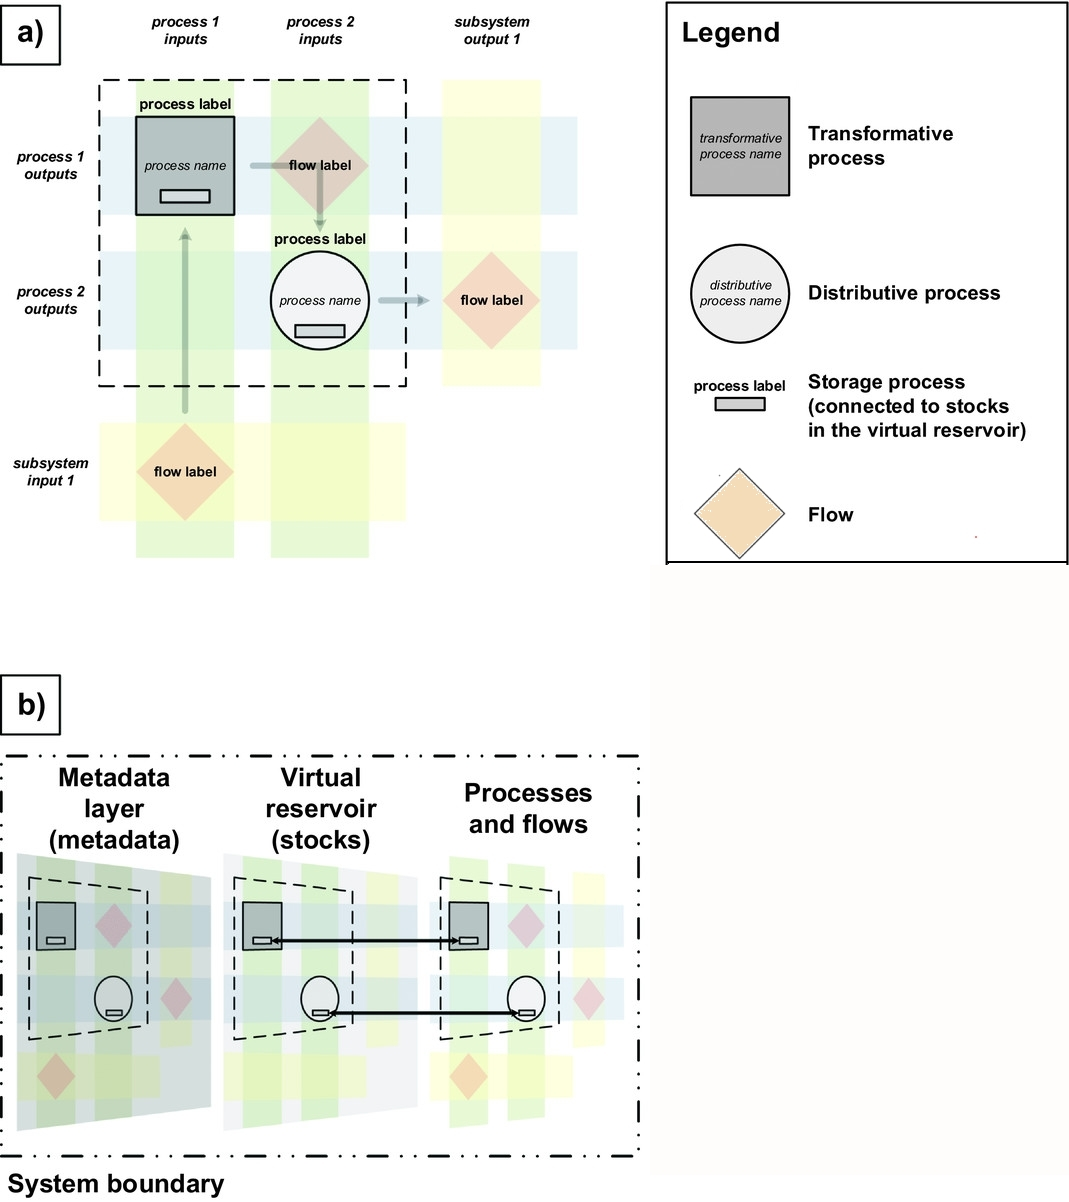
\includegraphics[width=0.6\textwidth]{images/umis_aspects.jpg}
\caption{(a) Key aspects of a UMIS diagram, visualizing it in a matrix style. Contains transformation, distribution and Storage processes as well as 3 flows. The processes lie on the diagonal and the flows are on the row of the origin process and the column of the destination process (b) The orientation of the virtual reservoir and metadata layer in reference to processes and flows. Flows depicted by grey arrows in (a) and conceptual linkages denoted by black arrows in (b) are for illustration and are not properties of UMIS diagrams. UMIS = Unified Materials Information System. Adapted from \cite{myers2019unified}}
\label{fig:umis_aspects}
\end{figure}

\subsection{Mass Balancing}
\label{sec:mass_balance}
MFA, IOA and LCA all share core modelling concepts. Each methodology involve a separation background and foreground systems, with the background system acting as a more generic supplier of inputs and outputs to the more detailed foreground system \cite{pauliuk2016prospective}. The foreground system is often modelled through a system of equations and constraints, but one common concept to all methodologies is that of mass balancing. The idea of this is that throughout the entire system, matter must be conserved. Therefore the total mass of a given material entering a process must be equal to the total mass leaving \cite{brunner2004practical}. This is defined by the following equation:

Where $i,j \in \{1,..,n\} $ are the processes in the system, $f_{ij}$ is a flow from process $i$ to $j$, $q_i$ and $o_i$ are the inflow and outflow between process $i$ and the background system respectively, and $\delta s_i$ is the stock being supplied to or coming from storage:     

\begin{equation}
    \label{eq:mass_balance_1}
    \forall i, q_i + \sum^{n}_{j}f_{ji} = \sum^{n}_{j}f_{ij} + o_{i} + \delta s_i 
\end{equation}

Further constraints can be supplied in the form of transfer coefficients which allocate the total amount of material flowing into the process amongst the flows leaving the process. With $a_{ij}$ being the transfer coefficient of the flow from process $i$ to $j$, $s_i$ is stock coming from storage (which may be 0) and $z_i$ as the total of all material entering process $i$, this can be defined as:

\begin{equation}
    \label{eq:mass_balance_2}
    z_i = q_i + \sum^{n}_{j}f_{ji} + s_i
\end{equation}

\begin{equation}
    \label{eq:mass_balance_3}
    f_{ij} = z_{i}a_{ij}
\end{equation}

Concentration equations can also be used when processes extract specific goods from substances. For example, in a system modelling the flow of iron, a process may be used to model the extraction of iron from iron oxide ore. This is denoted by the following equation where $f_s$ is the flow of substance $s$ (e.g iron oxide ore) into a process, $f_g$ is the flow of good $g$ (e.g iron) out of a process and concentration coefficient $c_{sg}$ is the concentration of good $g$ in substance $s$:

\begin{equation}
    \label{eq:mass_balance_4}
    f_s = f_g c_{sg}
\end{equation}

Whilst Myers et al. have demonstrated how material systems in LCA, MFA, IOA studies can be visualized as UMIS diagrams \cite{myers2019unified}, no work has be done to use UMIS structured data in a computational model. In order to demonstrate UMIS's suitability as a structuring system for data in a computational model I will develop a calculation engine for propagating uncertainty through UMIS structured systems.

\section{Uncertainty in IE}
\subsection{What is uncertainty?}
Common practice in IE research is to first define the system in terms of stocks, flows and processes and then identify values for the quantities of stock and flow. These observed values have an associated uncertainty which leads to an uncertainty in model outputs. As IE studies can be used to guide economic and political decisions, it is important to incorporate uncertainty into the results. A study by Danius and Burstr\"om \cite{danius2001regional} found that initial conclusions drawn when studying the flow of nitrogen were inconclusive when data uncertainties were taken into account. Therefore in cases where a comparison of systems are being conducted, the uncertainty around both systems must be taken into account to ensure that the results found are significant and cannot be attributed to variation in underlying data. As such, uncertainty is an important and well studied topic in the fields of LCA, IOA and MFA \cite{temursho201712, laner2014systematic, heijungs2004review}.

The sources of uncertainty can be separated into two kinds \cite{ferson1996different}. The first is aleatory uncertainty which comes from randomness in the underlying value. This is where either the method of measuring the value has an uncertainty around it so the precise value is unknown, or the value itself is non-deterministic. The second kind is epistemic which refers to generalizations about the value. One cause can originate from when values vary over space and time, therefore the value for a time period (e.g one year) or a geographic area (e.g the entire UK) can have an associated uncertainty. Another source can be subjective judgement such as when an unknown value is estimated based on a known value. Other causes can include scientific disagreement over the true value of a quantity, imprecise language on what the quantity refers to (e.g a material being said to be mostly carbon), and approximation in parameters in order to describe the system as a mathematical model. Epistemic uncertainty is potentially reducible through further investigation, however due to feasibility constraints it is sometimes unavoidable \cite{laner2014systematic}.

Further forms of epistemic uncertainty can be caused by possibilities in how the system is defined or described, however as we are looking at a general algorithm for propagating uncertainty in systems, this can be seen as out of scope. Instead, I will focus on uncertainty in specific parameter values.

\subsection{Incorporating Uncertainty into UMIS}
\label{sec:incorporating_uncertainty}
In \cite{laner2014systematic}, Laner et al. describe a five step procedure for incorporating uncertainty into MFA studies. These can be found in figure \ref{fig:incorp uncertainty procedure}:

\begin{figure}[t]
    \begin{enumerate}
        \item Establish mathematical model
        \begin{enumerate}
            \item Define system elements and relationships between the elements
            \item Define equations based on mass balance principle
        \end{enumerate}
        
        \item Characterize data uncertainty
        \begin{enumerate}
            \item Evaluate information about data (model parameters, inputs and outputs)
            \item Define characterising functions for uncertainty
        \end{enumerate}
        
        \item Combine data and mathematical model
        \begin{enumerate}
            \item Balance model and cross-check data
            \item Evaluate plausibility and reconcile data (iterative)
            \item Produce a calibrated model using all available data
        \end{enumerate}
        
        \item Calculate uncertainty for calibrated model
        \begin{enumerate}
            \item Propagate uncertainty through the model and calculate uncertainty of stocks and flows
            \item Interpret uncertainty estimates for resultant values from model 
        \end{enumerate}
        
        \item Analyze sensitivity \& develop scenarios
        \begin{enumerate}
            \item Identify critical model parameters
            \item Change parameters to perform scenario analysis
        \end{enumerate}
    \end{enumerate}
    \caption{Adapted from: \cite{laner2014systematic}}
    \label{fig:incorp uncertainty procedure}
\end{figure}

% 
As the MFA, IOA and LCA share constraints surrounding mass balancing in their system structure, steps 1-4 in the above procedure can be applied to all three methodologies. Where they diverge is in the fifth stage, where the model is used to calculate further values and perform analysis on the system. Therefore providing support for stages 1-4 can be seen as a relevant and useful addition to UMIS and STAFDB.

% IF you need to pad stuff out you can put another paragraph here about other ways they characterize uncertainty
UMIS provides a method for structuring stocks and flows data into the system described in step one of this procedure however does not explicitly specify a unified way for specifying how the uncertainty around data values must be described. Current development on STAFDB and in the Metabolism of Cities project favours an approach investigated by Laner in \cite{laner2016novel}. This strategy combines the use of a pedigree matrix to classify data quality, as defined by Weidema and Wesnaes \cite{weidema1996data}, and the application of data quality to uncertainty by Hedbrandt and S\"orme \cite{hedbrant2001data}. The pedigree matrix provides five criteria of data quality (reliability, completeness, temporal correlation and geographical correlation). When a data point is recorded it is given a score for each criteria. The score is combined with a sensitivity level to provide a coefficient of variation. The data point can then be modelled as a normally distributed random variable with a standard deviation related to its coefficient of variation. As stocks and flow values can never be negative and can have asymmetrical properties, it can be appropriate to model the data point as a log-normal random variable. Therefore Laner also provides a method for characterising data quality as an uncertainty factor which relates to the standard deviation of a log-normal distribution. Therefore Laner's work could be used to convert descriptions of a data point's uncertainty from quality scores to probability density functions.

% TODO talk about expert assumptions

Whilst the above approach provides a method for characterising the uncertainty of individual data points independently, it does not provide support for considering them in respect to the entire system. This is key to steps 3 and 4a of the procedure in figure \ref{fig:incorp uncertainty procedure}. To do this the data must be arranged as a mathematical model and the uncertainties of each model parameter must be calculated under the mass balance constraints. Typically this is performed using statistical approaches through either possibilistic methods, probabilistic methods or sensitivity analysis. 

As a single UMIS diagram structures data in terms of a single time snapshot, a useful addition to UMIS would be to provide a program to propagate uncertainty through a UMIS diagram and infer unknown stocks, flows and transfer coefficients. Programs to support analysis such as in steps 4b, and 5 or in situations unique to IOA and LCA would have to be unique to the study and therefore are out of scope for this thesis.

\begin{comment}
In \cite{lupton2018incremental}, Lupton et al. apply a Bayesian inference approach for propagating uncertainty through a model of plastic flows in Austria in 2005. In this paper, Lupton characterizes uncertainty of model parameters as normal distributions. I expand on this approach by generalising it to UMIS specified data and allowing for model parameters to be specified using log-normal distributions also.
 
\end{comment}

\section{Aims}
Below are the aims for this dissertation:

\begin{enumerate}
    \item Investigate literature in propagating uncertainty through industrial ecology models
    \item Develop a program to create a model from UMIS formatted data and propagate uncertainty through it
    \item Add support for representing uncertainty through normal, log-normal and uniform distributions
    \item Evaluate the accuracy and performance of the program
\end{enumerate}
\begin{comment}

Uncertainty
    - Why is it important to show uncertainty?
        - 
    - What are the methods for showing uncertainty?
    - Why is it important to hav a flexible method for showing uncertainty?
    - Need to show uncertainty
        - All studies are used to inform decision making
        - As such uncertainty has been the subject of various literature reviews in the fields of IOA, MFA and LCA, cite cite cite
        - Impairs reliability
        - Important when considering results
        - Can determine if results are significant compared to uncertainty
        - Environmental impacts and indicators are often calculated directly from    values, need to have accurate uncertainty around those values in order to   confidently talk about environmental impact
    - Sources of uncertainty
        Because IE studies often work on an average (i.e average amount of copper, average amount of zinc flowing through)
        
        read this one, take notes, read the lca one quickly, take notes, see how IOA one is important
    - Methods of dealing with and calculating uncertainty
        - Talk about 2 things that aren't related to probabilistic
        - Talk about the Fuzzy set theory, sensitivity analysis, stan, probabilistic and then lupton and then say where mine fits in 
    - Reliability scores (talk in regards to STAFDB and UMIS, ecoinvent scores)
        - Useful when integrating data from across studies
        - Need for lognormal
        - Need to ensure that consistency is kept according to the later laner paper
  
 - Transformation processes have only one outflow
 - Visualized here as a matrix
- Metabolism of Cities
    - Digital research lab created by Paul Hoekman designed to store and facilitate Industrial Ecology research.
    - Contains a store of publications, IE data and an online material flow analysis tool that is designed to allow users to easily conduct MFA studies and interface with an online database.
    - Its primary aim is to encourage and allow collaboration between researches to fully undertand the metabolism of resources and energy surrounding specific regions.
    - Current
- Industrial Ecology
    What is it
    What methods does it use
        LCA
        IOA
        MFA
- STAFDB
   - over the past 20 years the graedal research group at yale university have compiled Industrial Ecological data covering over 60 chemical elements and over 100,000 data entries
   - The data from this has been extracted and placed into YSTAFDB, currently work is continuing to develop STAFDB, a community driven database that enhances YSTAFDB by making it more user friendly and dealing with problems related to divergent disaggregation.
   Disaggregation is where a classification of data is separated into its constituent parts. For example data about cars could be separated into electric or non-electric vehicles as well as large cars or small cars. If two studies were to disaggregate data in different ways, data about the same objects may be counted twice when structured into the same system 
   -UMIS provides a way for structuring YSTAFDB data in a methodology agnostic manner, by enforcing the data to be structured in a directed bipartite graph as well as including a separator flag for processes and materials to ensure that divergent disaggregation is detected.
   - 2 dimensions of edges, one for the tree another for the system (graph)
   - Matrix and layers
- UMIS
 - Ontology
 - What UMIS does
 - Vocabulary based on MFA
 - Allows for dissagregation
 - Difference between communication diagrams and UMIS
 - Each study can still have its own communication diagrams
 - The data can also be represented in a UMIS diagram and stored in a common DB
 - This allows data to be shared between studies
 - Nulius in verba: Can store data online for transparancy
 - Components of a umis diagram (basically only need to say its a directed bipartite graph
 - Talk about MFA terminology
  - Talk about stafdb
 - You're focusing on how this thing is relevant
 -  
- Metabolism of Cities
- Uncertainty
    - Uncertainty scores
    - Ecoinvent
    - Need to be able to flexibly support different forms of uncertainty
   
- No work as of yet has been done to use UMIS as a feed in for a computational model
-   
    
- Show how data referenced in UMIS can be referenced in databases and computational models
    - 
- What is the project topic or problem being investigated?
- Why is the topic important, why should the reader care about it?
- What are the central challenges involved and why are they significant?
\end{comment}



% -----------------------------------------------------------------------------

\chapter{Technical Background}
\label{chap:technical}
There are a variety of different methods for propagating uncertainty throughout MFA models. These typically fall under four main approaches, Guassian error propagation, possibility theory, probability theory and sensitivity analysis. \cite{laner2014systematic}. Uncertainty propagation can also be seen to involve three tasks, that of data reconciliation, error propagation, and data model consistency.

Data reconciliation involves altering data values so that they agree with all constraints in the mathematical model. As the data values are inherently uncertain, cases occur where their most likely values do not satisfy mass balance constraints, but one of their possible values do. For example take three flows $A, B$ and $C$ where flows $A$ and $B$ are entering a process and flow $C$ is leaving. The mass balance equation is $A + B = C$. Say we model our prior uncertain knowledge of each flow by representing each as a random variable where $A \sim \mathcal{N}(30, 10^2)$, $B \sim \mathcal{N}(5, 2^2)$ and $C \sim \mathcal{N}(32, 4^2)$. As the expected values $A = 10, B = 5, C = 32$ do not satisfy the mass balance constraint, we can use our prior knowledge of the data values and the knowledge of how the material should behave in the system to reduce the uncertainty of all three parameters to a point where their expected values all agree with the constraint.

% Image of data reconciliation
Error propagation involves inferring the uncertainties of values calculated by the model using the uncertainties of parameters supplied to the model. An example would be inferring the expected value and standard deviation of flow $C$ in the above case.

Cases can occur when the independent data values obtained from the model do not agree at all with the model structure. The degree to which how well the data agrees with the model is known as data model consistency. A model which is completely consistent will have prior data values that agree with the mass balance constraints whilst a completely inconsistent model will have no way of reconciling the data so that agreement is reached. Between these two extremes are where values had to be reconciled to move into agreement.

As the mathematical model involves linear (Eqs. \ref{eq:mass_balance_1}, \ref{eq:mass_balance_2}) and non-linear (Eqs. \ref{eq:mass_balance_3}, \ref{eq:mass_balance_4} constraints, situations arise where two uncertain and therefore variable parameters are multiplied together. This adds greater complexity to the task.

\section{Sensitivity Analysis}
A more model specific approach to propagating uncertainty is that of sensitivity analysis \cite{laner2014systematic}. This technique puts a focus on evaluating the effect of a specific parameter's uncertainty on the model's results. The parameter is varied throughout its possible values and the different result values are recorded, producing an uncertainty interval for the results. This can be repeated for multiple parameters to try and identify what has the greatest effect on the results and therefore identify "hotspots" where changes in the real world should be enacted. This approach is less general than other approaches to dealing with uncertainty and therefore is not appropriate for an integration into a general system such as UMIS.

\section{Gaussian Error Propagation}
Gaussian Error Propagation is used by STAN, a free software for performing MFA \cite{cencic2008material}, developed by Oliver Cencic. STAN provides a GUI for creating graphical MFA models comprising of stocks, flows and processes. The graphical model is translated into a mathematical model using equations \ref{eq:mass_balance_1}, \ref{eq:mass_balance_2}, \ref{eq:mass_balance_3} and \ref{eq:mass_balance_4}. Each parameter in this equation may be considered to be unknown (\pmb{$y$}), known with an uncertainty (\pmb{$x$})  or exactly known (\pmb{$z$}). Uncertainty is characterised by STAN through the use of 68 \% confidence intervals around a "true" value. This is modelled as a normally distributed random variable with the "true" value as the mean ($\mu$) and the 68\% confidence intervals as the standard deviation ($\sigma$).

In STAN, uncertainty propagation is performed in two stages \cite{cencic2016nonlinear}. First \pmb{$x$} are reconciled giving a new mean and standard deviation for each parameter (\pmb{$\mu^*$} and \pmb{$\sigma^*$}). Next, the unknown parameters are calculated from \pmb{$\mu^*$} and \pmb{$\sigma^*$} of known values. It is possible to also calculate the confidence interval of the unknown values, as all uncertainties are assumed to be modelled as normal distributions. This allows for uncertainty to be propagated to model results. By measuring the distance each parameter has been reconciled from its original value, we can get a measure of data-model consistency. We can impose a limit relative to a data value's variance to determine when a data point has been reconciled so far that the model can be seen to no longer be in agreement.

Data reconciliation is performed in the form of a weighted least squares optimization problem. The optimization is of minimizing the objective function \ref{eq:objective_function}: 

\begin{equation}
\label{eq:objective_function}
    F(\pmb{\mu^*}) = (\pmb{\mu} - \pmb{\mu^*})^T \pmb{\mathcal{Q}}^{-1}(\pmb{\mu} - \pmb{\mu^*})
\end{equation}

Where $\mathcal{Q}$ is a matrix containing the confidence intervals of the known parameters on the diagonal. $\mathcal{Q}$ provides weightings in this minimization resulting in the more uncertain parameters being reconciled "further" than the more certain parameters. 

The minimization of the objective function \ref{eq:objective_function} is done in respect to mass balance constraints obtained from the graphical model. These equations may be non linear as they can involve flow parameters being multiplied with transfer or concentration coefficient parameters. The constraints of the objective function must be in linear form, therefore a linear approximation of the mass balance is obtained using a first order Taylor series expansion on the on-linear constraints. Full details can be found in \cite{cencic2016nonlinear}. 

The advantages of using this approach is that it is relatively fast in comparison to Bayesian approaches. It also performs validation to ensure that all unknown parameters can be inferred by the algorithm and does not try to calculate them if not enough known parameters are supplied. This is done by using Guassian elimnation to convert the set of constraint equations into reduced row echelon form. This allows you to check certain rows of the matrix to ensure that there exists at least one equation with only one unknown parameter for each unknown parameter.

Disadvantages to this approach is that it enforces all uncertainty to be characterised as normal distributions. This has shown to be too restrictive for a great deal of IE applications in section \ref{sec:incorporating_uncertainty}. The data reconciliation algorithm has also been shown to fail when parameters in non-linear equations are modelled to have a large uncertainty. To allow for more flexible and robust representations of uncertainty, possibilistic or probabilistic approaches should be used instead.
%TODO fix minimization and optimization
\section{The Possibilistic Approach}
% Image of fuzzy interval/membership function
Possibilistic approaches are based on fuzzy set theory where model parameters and their uncertainty are represented by fuzzy sets. A fuzzy set is used to model a "vaguely perceived or imprecisely defined quantitative piece of information" \cite{dubois2000fuzzy} and involves a membership function which maps a value to the degree to which the value belongs in the set: $f: X \rightarrow{[0,1]}$. Intersection, union, addition and subtraction operations are supported over fuzzy sets \cite{viertl2006beschreibung}. Model parameters are represented by special cases of membership functions where $X = \{x | x \ge 0\}$, and $x$ is mapped to the likelihood the parameter would take that value. D\v{z}ubur et al. propose a data reconciliation and error propagation algorithm using fuzzy sets and demonstrate it on a case study of the Austrian wood system in 2011 \cite{dvzubur2017fuzzy}. In this study, the uncertainty of the $m$ prior known model parameters ($x \in \{x_1, .. x_m\}$) are characterised through trapezoidal or triangular membership functions, but can be arbitrary as long as they are convex and normalised to 1. In cases where there a multiple data sources for a parameter, $x_i$ it is defined by the intersection of each data source's membership function.

%% PCITURE OF INTERSECTION OF FUZZY INTERVALS
The fuzzy set theory approach deals with non-linear operations first before reconciling values according to linear constraints. Membership functions for each stock or flow in the model are calculated from the prior known values, these can be already known or may have to be calculated through non-linear operations. If stocks or flows are specified in multiple ways then the intersection of the membership functions is used. This step results in $n$ model parameters ($\hat{x} \in \{x_1, .. x_n\}$).

Next  D\v{z}ubur et al. present a 3 step procedure for reconciling stock and flow values using the mass balance constraints (Eq. \ref{eq:mass_balance_1}) around each process. Their procedure makes a distinction between internal flows (flows between processes in the model) and external flows (flows between a process and outside the model). We will refer to both stock and flows as flows for the procedure:

    \begin{enumerate}
        \item Calculate each internal flow $i$, as 3 different membership functions ($\gamma_1, \gamma_2, \gamma_3$)
        \begin{itemize}
            \item $\gamma_1 := \hat{x}_i$ 
            \item $\gamma_2 := $ mass balancing the origin process of the flow using    $\hat{x}$
            \item $\gamma_3 := $ mass balancing the destination process of the flow using $\hat{x}$
            \item $\bar{x}^*_i := $  $\cap(\gamma_1, \gamma_2, \gamma_3)$
            \item $\alpha_{i} := $ the peak of $\bar{x}^*$
        \end{itemize}
        
        \item Calculate each external flow $j$, as 2 different membership functions ($\gamma_1, \gamma_2$)
        \begin{itemize}
            \item $\gamma_1 := \hat{x}_j$ 
            \item $\gamma_2 := $ mass balancing the internal process of the flow using $\hat{x}$ (for other external flows) and $\bar{x}^*$ (for internal flows)
            \item $\bar{x}^*_i := $  $\cap(\gamma_1, \gamma_2)$
            \item $\alpha_{j} := $ the peak of $\bar{x}^*$
        \end{itemize}
        
        \item Each $\gamma^*$ is normalised to 1
    \end{enumerate}

As a result of this procedure we have the reconciled and calibrated data values with respect to constraints $\hat{x}^*$ as well as a global measure of data-model consistency as the minimum $\alpha$ value. This $\alpha$ value provides validation for the model as if it is 0 at any intersection there is explicit information that there is either a problem with the data values defined or the way the model has been structured.

The running time of this method is relatively low at $O(n*d)$ where $d$ is a variable related to the number of "cuts" of a membership function used when performing operations on membership functions. This therefore appears faster than the Gaussian error propagation algorithm which requires the Gaussian elimination and therefore has at least $O(n^3)$ time. The two are not directly comparable however as the fuzzy set approach requires the model of constraints to be stated explicitly, whilst the algorithm employed by STAN automatically develops a mathematical model.

Whilst fuzzy sets are one method of representing the uncertainty around data values, they are limited in that they are forced to be bounded. Therefore they struggle to represent the far tail end of values which may result in unlikely scenarios. By basing the representation on arbitrary probability density functions (pdfs) such as those used in Bayesian inference approaches, you have greater flexibility in how you choose to characterise uncertainty.  
% States how to do it explicitly, doesn't provide an algorithm for doing it automatically

\section{Probabilistic approaches}
Another tactic for propagating uncertainty throughout a model is using pdfs. Whilst the Guassian error propagation approach propagates uncertainty when assuming normal distributions, this provides an inflexibility over how uncertainty can be characterised. The need for both normal and log-normal distributions can be seen by Laner's work as discussed in section \ref{sec:incorporating_uncertainty}, but many studies characterise uncertainty of parameters through a wide variety of probability distributions\cite{wernet2016ecoinvent, gottschalk2010probabilistic}, including triangular, trapezoidal and uniform. The uncertainty represented by these distributions needs to be calibrated to the mass balance constraints from the structure of the model as well as propagated to any model results by calculating their pdfs. Pdfs are more informative than using just mean and variance or fuzzy sets as metrics such as percentiles, skewness and correlation between parameters can be calculated.

\subsection{Monte Carlo Simulations}
In \cite{gottschalk2010probabilistic}, Gottschalk et al. explores a probabilistic approach to model uncertainty in a MFA study investigating the environmental exposure of nano-particles. This mathematical model was built in terms of inflows to the system and transfer coefficients between processes in the system. Uncertainty of the inflows was characterised with a lognormal distribution and the transfer coefficients with triangular and uniform distributions. Stocks and flows values were seen as the results of the system and were calculated through matrix algebra.

External inputs to the system were organised into a column vector $\mathbf{q} \in \mathbb{R}^{n \times 1}$ where $q_i$ is the amount of material flowing into process $i$. Transfer coefficients were arranged into a matrix $A \in \mathbb{R}^{n \times n}$ where $t_{ij}$ is the transfer coefficient for the flow from process $i$ to $j$ (see Eqs. \ref{eq:mass_balance_2} \& \ref{eq:mass_balance_3}). The unknown total flow into each process $z_i$ was arranged as $\mathbb{z} \in \mathbb{R}^{nx1}$. The mass balance constraints were enacted as:

\begin{equation}
\label{eq:gottschalk_eq}
    (I-A)\bm{z} = \bm{q}
\end{equation}

Where $I$ is the $n \times n$ identity matrix.

Monte Carlo (MC) simulations were used to calculate pdfs for the stock and flow values of the results with $r=100,000$ samples. $r$ values for each transfer coefficient $a \in A$ are sampled from their pdfs. The values are used to calculate corresponding stock and flow values by solving for the total flow into a process, $\bm{z}$ and substituting that in equation \ref{eq:mass_balance_3}. Pdfs of the stocks and flows that account for the uncertainty in the model inflows and transfer coefficients can then be constructed from their $r$ samples. Whilst this technique does generate pdfs of stock and flow values when transfer coefficients are known, it does not incorporate any prior knowledge of the stocks and flows values. To accomodate this, Gottschalk et al. extended this approach with Bayesian inference.

\subsection{Bayesian Inference}

Bayesian inference is a technique that can be used to infer pdfs of model parameters in non-linear systems \cite{green2015bayesian}. When building an MFA system you implicitly define prior knowledge about the parameters within it. This may come from the system structure in the form of dependencies from mass balance constraints, or from a prior belief of a range parameter will lie in. For example when modelling a system, the researcher will know a flow value will be somewhere between 0 and the total input into the system. Once a MFA model has been converted into a mathematical model $I$, the joint prior probability distribution of the model parameters can be written as $P(\theta|I)$. As we have seen, model parameter values may be measured or estimated with an uncertainty ($D$). Bayes theorem allows us to infer the pdfs of reconciled model parameters (or \textit{posterior} $P(\theta | D, I)$) given the \textit{likelihood} of observations of parameter values \cite{lupton2018incremental}:

\begin{equation}
    \label{eq:bayes_theorem}
    p(\theta | D) = \frac{p(D | \theta, I)p(\theta|I)}{p(D | I)}
\end{equation}

where the denominator (the marginal likelihood) is defined as:

\begin{equation}
    \label{eq:marginal_likelihood}
    p(D| I) = \int{}{}p(D|\theta, I) p(\theta| I)d\theta 
\end{equation}

% Explain these equation terms fully in the implementation section
This allows us to calculate the pdfs of each parameter value weighted by to the likelihood of these observations. As the number of model parameters can often be large it can be complex to calculate the marginal likelihood, but by using Monte Carlo Markov Chain (MCMC) algorithms we can generate samples from the posterior distribution and use those samples to infer the posterior distributions of model parameters.

\subsubsection{Monte Carlo Markov Chain Algorithms}
Monte Carlo Markov Chain algorithms are techniques which allow for sampling from unknown posterior distributions. Basic MCMC algorithms require two things. The first is a  proposal distribution ($g(\theta)$) for the model parameters. The second is a distribution proportional to the posterior distribution \cite{green2015bayesian}. As the denominator in equation \ref{eq:bayes_theorem} is constant for all model parameters, our proportional distribution is:

\begin{equation}
    \label{eq:proportional_dist}
    f(\theta) =  p(\theta|I) p(D | \theta, I) \propto p(\theta | D)
\end{equation}

or the probability of observing the data given the model multiplied by the prior \cite{lupton2018incremental}. MCMC algorithms construct a Markov Chain with a stationary distribution equivalent to the target posterior density. This is done by drawing a proposal sample vector of of all parameters in the model $\bm{\theta}^*$ from $g\bm{\theta}$ and using an acceptance probability to determine if the sample is representative of the posterior distribution. The acceptance probability is:

\begin{equation}
    \alpha(\bm{\theta}^i, \bm{\theta}^{i-1}) = min (1, \frac{f(\bm{\theta}^i)g(\bm{\theta}^{i-1})}{f(\bm{\theta}^{i-1})g(\bm{\theta}^{i})})
\end{equation}

Therefore the probability of being accepted is proportional to how likely the new proposal belongs to the posterior compared to the the previous proposal. By using the ratio: $\frac{f(\bm{\theta}^i)}{f(\bm{\theta}^{i-1})}$ and using equation \ref{eq:bayes_theorem}, we can see that the marginal likelihood constant cancels. Algorithm \ref{alg:monte_carlo} shows a procedure for obtaining samples of model parameters from their posterior distribution.

\begin{algorithm}[]
    \For{$i = 1$ to $n$ samples}{
        Draw candidate vector of proposal parameters $\bm{\theta}^*$ from $g(\bm{\theta})$\;
        Compute acceptance probability $a = \alpha(\bm{\theta^*}, \bm{\theta}^{i-1})$\;
        Draw uniform random number $u \in[0,1]$\;
        \eIf{$u \le a$}{
            Accept $\bm{\theta}^*$\;
            Store $\bm{\theta}^*$\;
            $\bm{\theta}^i = \bm{\theta}^*$\;
        }{
            Reject $\bm{\theta}^*$\;
            Store $\bm{\theta}^{i-1}$\;
            $\bm{\theta}^i = \bm{\theta}^{i-1}$
        }
    }
    \caption{Monte Carlo Markov Chain Sampler}
    \label{alg:monte_carlo}
\end{algorithm}

Gottschalk et al. use such a sampler to improve on their Monte Carlo simulation results. However, due to a scarcity of nano-particle data, Gottschalk et al. had to estimate values for their observations of stocks and flows values. Because of this, they did not provide the likelihood functions of their model parameters for their MCMC sampler, only describing the approach they used and presenting their more certain, posterior distributions for stock and flow values.

\subsubsection{Independence Sampler}

In \cite{cencic2018data, cencic2015general}, Cencic improves on his Gaussian propagation approach by describing a Bayesian framework for data reconciliation over MFA models. His approach involves using the observations of all model parameters as priors and then inferring the posterior distribution of those parameters when constrained by the mass balance equations. Therefore this method differs from that of Gottschalk as the posterior is not inferred from the likelihood of an observation, but from using the mass balance constraints. In his technique he divides model parameters into three groups:

\begin{itemize}
    \item $\bm{w} \in W^{n_w}$ - Observed free variables, model parameters with a known prior distribution $p_w(\bm{w})$
    \item $\bm{u} \in U^{n_u}$ - Observed dependent variables, model parameters with a known prior distribution $p_u(\bm{u})$ that are functions of $\bm{w}$
    \item $\bm{y}$ - Unobserved dependent variables, results of the model calculated from model parameters
\end{itemize}

The functions that define the dependent variables are $\bm{u} = \bm{h}(\bm{w}) = \begin{bmatrix}
    h_1(\bm{w}) \\
    \vdots \\
    h_{n_u}(\bm{w})
\end{bmatrix}$

and $\bm{y} = \bm{h}(\bm{w})$. Therefore $\bm{h}(\bm{w})$ can be thought of as $n_u = |\bm{u}|$ non-linear or linear constraint equations. Cencic also introduces the concept of a constraint manifold. If model parameters $\bm{w}$ and $\bm{u}$ can be thought of as having an independent joint prior pdf in a space $D \subseteq \mathbb{R}^{n_w + n_u}$, the model equations can be seen to define a constraint manifold $S \subset D$ where the equations are satisfied and model parameters are valid. Therefore the posterior distribution of model parameters conditional on model equations ($\pi_s(\bm{w})$) is the pdf of $S$. Cencic uses the example shown in figure \ref{fig:cencic_manifold} where $\bm{w} = \begin{bmatrix}
    x_1 \\
    x_2
\end{bmatrix}$
, $\bm{u} = [x_3]$ and $\bm{h}(\bm{w}) = [h_{x_3}(\bm{w})] = [x_1 + x_2]$, as a visualisation of $S$ as a plane. By using a MCMC sampler, the posterior distribution of $S$ can be inferred using proposals of $\bm{w}$. The accepted values for $\bm{w}$ can be used then to calculate the dependent variables.

The MCMC sampler described is known as an independence sampler as its proposals for $\bm{w}$ are drawn independently from their marginal distributions, $g(\bm{w}) = p_w(\bm{w})$. The proportional distribution $f(\bm{w}^{i}, \bm{w^{i-1}}$ of the sampler must be proportional to the pdf of the constraint manifold $S$. As prior distributions of $\bm{u}$ and $\bm{w}$ are assumed to be independent, $\pi_s(\bm{w}) = \frac{p_{u}(\bm{h}(\bm{u}) p_{w}(\bm{w}) V(\bm{w}}{\int_W p_{u}(\bm{h}(\bm{u}) p_{w}(\bm{w}) V(\bm{w}) d\bm{w}}$. The term $V(\bm{w}) = \sqrt{|I + \bm{H}^T\bm{H}|}$ is a Lebesgue measure of the constraint manifold $S$ where $\bm{H} = \begin{bmatrix}
    \frac{\partial h_1{\bm{w}}}{\partial w_1} & \dots & \frac{\partial h_1{\bm{w}}}{\partial w_{n_w}} \\ 
    \vdots & \ddots & \vdots \\
    \frac{\partial h_{n_u}{\bm{w}}}{\partial w_1} & \dots & \frac{\partial h_{n_u}{\bm{w}}}{\partial w_{n_w}} \\
\end{bmatrix}$ and is evaluated at $\bm{w}$.
%If you need to pad you can add a bit about the non-linear and linear stuff
\begin{figure}[]
\centering
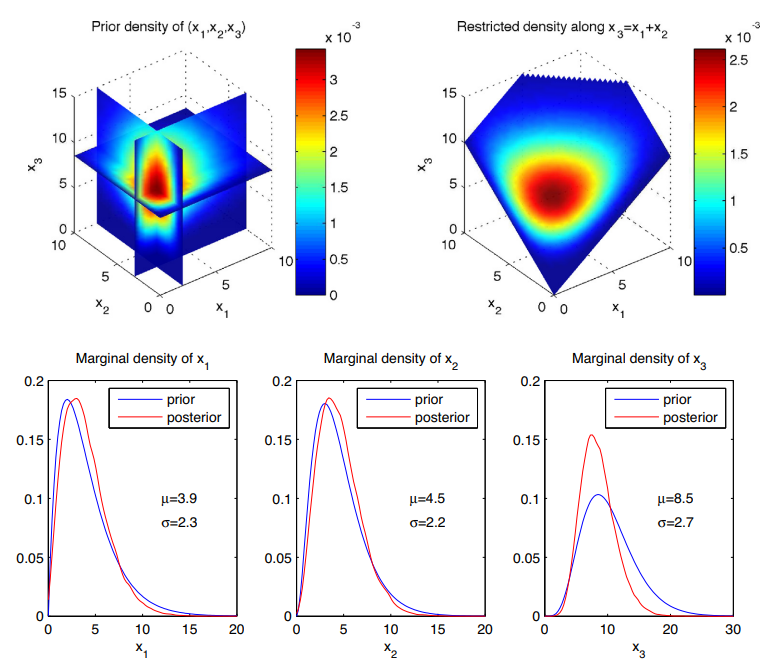
\includegraphics[width=0.5\textwidth]{images/cencic_manifold.png}
\caption{Visualisation of prior distributions with constraint manifold. Top left: prior pdfs of observed variables. Top right: Pdf of variables under constraints. Bottom: Marginalised densities of variables under constraints. Source: \cite{cencic2015general}}
\label{fig:cencic_manifold}
\end{figure}

%TODO maybe write a bit about how the acceptance proposal pushes towards a stationary distribution for the markov chain

In his paper, Cencic evaluates his approach over small MFA models of at most two processes where the functions $\bm{h}(\bm{w}$) are calculated explicitly. Therefore, in generalising it to generic MFA models, a system must be created for selecting which observed variables are to be considered free and which are dependent. Another task is the construction of $n_u$ constraint functions, which incorporate all the mass balancing information to express each dependent variable.

\subsubsection{Incremental MFA}
In \cite{lupton2018incremental}, Lupton presents an incremental approach to reducing uncertainty in an MFA model tracking the flow of steel in Austria in 2015. The external inputs $\bm{q}$ and transfer coefficients $\bm{A}$ can be thought of as free variables, and observations of a subset of the flow parameters as dependent variables. This approach did not attempt to infer the posterior distribution of a constraint manifold, but rather uses the likelihood of dependent observations to accept or reject free variable proposals. Characterisations of flow value observations as normally distributed random variables were used to model the likelihood of dependent flows belonging to the observed distribution. A full description of the construction of the model can be found in section \ref{sec:model_construction}. To construct their model and perform the MCMC sampling, Lupton used a variation of a Hamiltonian Monte Carlo sampler called the No-U-Turn (NUTS) sampler, provided by pymc3 \cite{salvatier2016probabilistic}.
% Lupton presents incremental MFA
% Free variables are input * tc in manner of gottschalk, used to create dependent observed variables of flows
% Calibrate parameters with observations of flows
% Uses NUTS sampler which hides away most of the specifics

% TODO put correct section ref thing here
% TODO check that I either always say variables or parameters

\subsubsection{Hamiltonian Monte Carlo and the No-U-Turn sampler}
Hamiltonian Monte Carlo (HMC) \cite{betancourt2017conceptual} provides a useful method for sampling a new proposal vector sample from the previous accepted proposal. The Hamiltonian sampler can be though of treating the multi-dimensional posterior distribution of model parameters as a concave surface and its log likelihood as a negative potential energy function. An accepted proposal parameter $\theta^i \in \bm{\theta}^i$ can be thought of as a coordinate on that surface with $r$ the momentum of a particle at that coordinate. $L$ "Leapfrog" steps (shown in algorithm \ref{alg:leapfrog}) calculate a new proposal parameter $\theta^{*}$ from $\theta^{i-1}$ by "rolling" this "particle" along the surface with momentum $r$ and distance $\epsilon$. To ensure variation in the next parameter proposed, $r$ is initialised randomly before performing the leapfrogging steps.

\begin{figure}[]
\centering
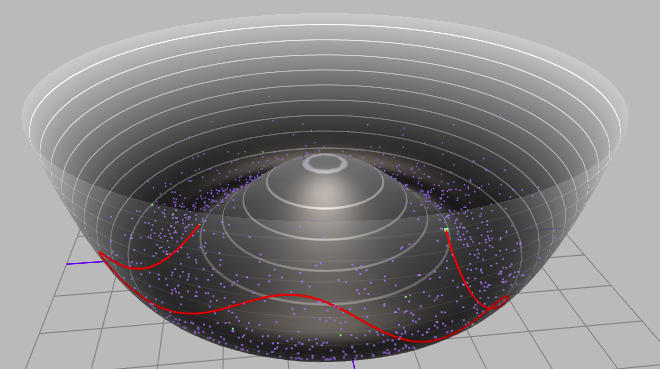
\includegraphics[width=0.5\textwidth]{images/hamiltonian_mcmc.png}
\caption{Visualisation of Hamiltonian Monte Carlo Sampling along a 2-Dimensional posterior probability density function. The red line shows the leapfrogging step from the previous accepted proposal value, the green box. Source: \cite{rogozhnikov_2016}}
\label{fig:umis_aspects}
\end{figure}

\begin{algorithm}[]
Given $\bm{\theta}, r, \epsilon$\;
\;
Set $\Tilde{r} = r + (\epsilon/2)\Delta_\theta\mathcal{L}(\theta)$\;
Set $\Tilde{\theta} = \theta + \epsilon \Tilde{r}$\;
Set $\Tilde{r} = r + (\epsilon/2)\Delta_\theta\mathcal{L}(\Tilde{\theta})$\;
\textbf{return} $\Tilde{\theta}, \Tilde{r}$\;
\caption{Leapfrog step: \newline Finds new proposal parameter $\Tilde{\theta}$ from previous parameter $\theta$, with previous momentum $r$, step size $\epsilon$ and log-likelihood of posterior distribution $\mathcal{L}$}
    \label{alg:leapfrog}
\end{algorithm}

$L$ and $\epsilon$ must be tuned correctly during the algorithm to ensure efficient sampling. If $\epsilon$ is too large, the proposal vectors drawn will have been drawn too far away from the previous value and therefore will be rejected too often, wasting computation time. Also if $L$ is too large, the leapfrogging will perform a "U-Turn" and start moving $\theta$ towards its original value. If $L$ and $\epsilon$ are too small then the proposed values will be too similar to each other and therefore not explore the full space of the posterior distribution. The No-U-Turn sampler (NUTS) \cite{hoffman2014no} automatically tunes $L$ and $\epsilon$ to avoid these issues.

In this thesis, I will use adapt Lupton's approach to  propagating uncertainty through MFA models for UMIS structured systems. This technique will involve automatically developing a mathematical model from a system defined by stocks and flows with independently observed data values and then using a NUTS sampler provided by pymc3 to infer the posterior distributions of these values in respect to mass balance constraints over the model. 
%TODO get rid of all yous, make first person
% Lupton models the parameters as dependent on the input parameters
\begin{comment}
 - Talk about other approaches for dealing with 
 - Pymc3
  - Lupton
  - Cencic/Stan
  - Cencic offer simplex algorithms as a way for automatically constructing the model but do not implement a program to do so
  - Bayesian Inference
  - A fuzzy set-based approach to data reconciliation in material flow modeling,
        - Can talk about this, can suggest that using probability distributions is better because fuzzy sets have trapezoidal and triangular membership functions which can be modelled as distributions if you use pymc3 correctly
  - we want a general approach to specifying the outputs of the model
  - Probibilistic is flexible to all kinds of uncertainty characterization, intervals can be expressed as uniform, normal, triangular, trapezoidal distributions exist, can show long tail
  - Pymc3 allows specification of their own distributions through interpolated, can construct a triangular or trapezoidal distribution from those
  
  - So its good that you've studied this stuff because you'll want to talk about it in the technical thing
  - First read other technical things and see if they are similar
  - I think for the technical thing the topics are
    - AISHA, read that to see if they indicated a good way to explain the ways that   they built the constraints automatically
    - Fuzzy set theory method 
    - STAN method
    - Mathematical MFA method
    - Sensitivity analysis method
    - Probabilistic MFA, what I use
    - Monte Carlo Markov Chains
    - No-U-Turn, metropolis hastings
    - Pymc3
    
    
\end{comment}



% This chapter is intended to describe the technical basis on which execution
% of the project depends.  The goal is to provide a detailed explanation of
% the specific problem at hand, and existing work that is relevant (e.g., an
% existing algorithm that you use, alternative solutions proposed, supporting
% technologies).  

% Per the same advice in the handbook, note there is a subtly difference from
% this and a full-blown literature review (or survey).  The latter might try
% to capture and organise (e.g., categorise somehow) {\em all} related work,
% potentially offering meta-analysis, whereas here the goal is simple to
% ensure the dissertation is self-contained.  Put another way, after reading 
% this chapter a non-expert reader should have obtained enough background to 
% understand what {\em you} have done (by reading subsequent sections), then 
% accurately assess your work.  You might view an additional goal as giving 
% the reader confidence that you are able to absorb, understand and clearly 
% communicate highly technical material.

% -----------------------------------------------------------------------------

\chapter{Project Execution}
\label{chap:execution}

\section{Overview}
The aim for this thesis is to prove UMIS's suitability as a basis for performing computation over industrial ecology systems. To show this I have developed a Bayesian inference engine to propagate uncertainty through UMIS systems and display the calibrated uncertainty values for stocks and flows data. This task is formed of three sections:

\begin{enumerate}
    \item Extract stocks and flows data from STAFDB and arrange in a UMIS diagram
    \item Convert the UMIS diagram into a mathematical model and propagate uncertainty through it
    \item Display calibrated uncertainty values for stocks and flows data
\end{enumerate}

% The aim for this thesis is to prove UMIS's suitability as a basis for performing computation over industrial ecology systems. To show this I have developed a Bayesian inference engine to propagate uncertainty through UMIS systems and display the calibrated uncertainty values for stocks and flows data. As STAFDB has yet to be publically released, I have developed a prototypical version as a series of CSV files. Information provided by Rupert Myers and Zo\"e Petard from the University of Edinburgh has ensured that the prototype has a similar structure to the version under development. I then extract the stocks and flows data and represent them as a UMIS diagram with python objects. I then convert the UMIS diagram into a mathematical model and infer calibrated uncertainty values as histograms for the stocks and flows data using MCMC sampling. Calibrated uncertainty values can then be estimated from the histogram data.

\section{Constructing the UMIS diagram}
% Construction of UMIS diagrams involves the extraction of data from STAFDB and then structuring them as a socioeconomic system

\subsection{STAFDB Prototype}
\label{sec:prototype_stafdb}
As STAFDB has not yet been released, I have developed a prototypical version (STAFDB-P) for my implementation. I was provided an Entity Relationship Diagram (ERN) for in-progress STAFDB by Zo\"e Petard from the University of Edinburgh. As only a subset of the entities in the database are necessary for the inference engine, the STAFDB-P only contains that subset. An ERN describing the prototype can be seen in figure \ref{fig:prototype_ern}.

\begin{figure}
    \centering
    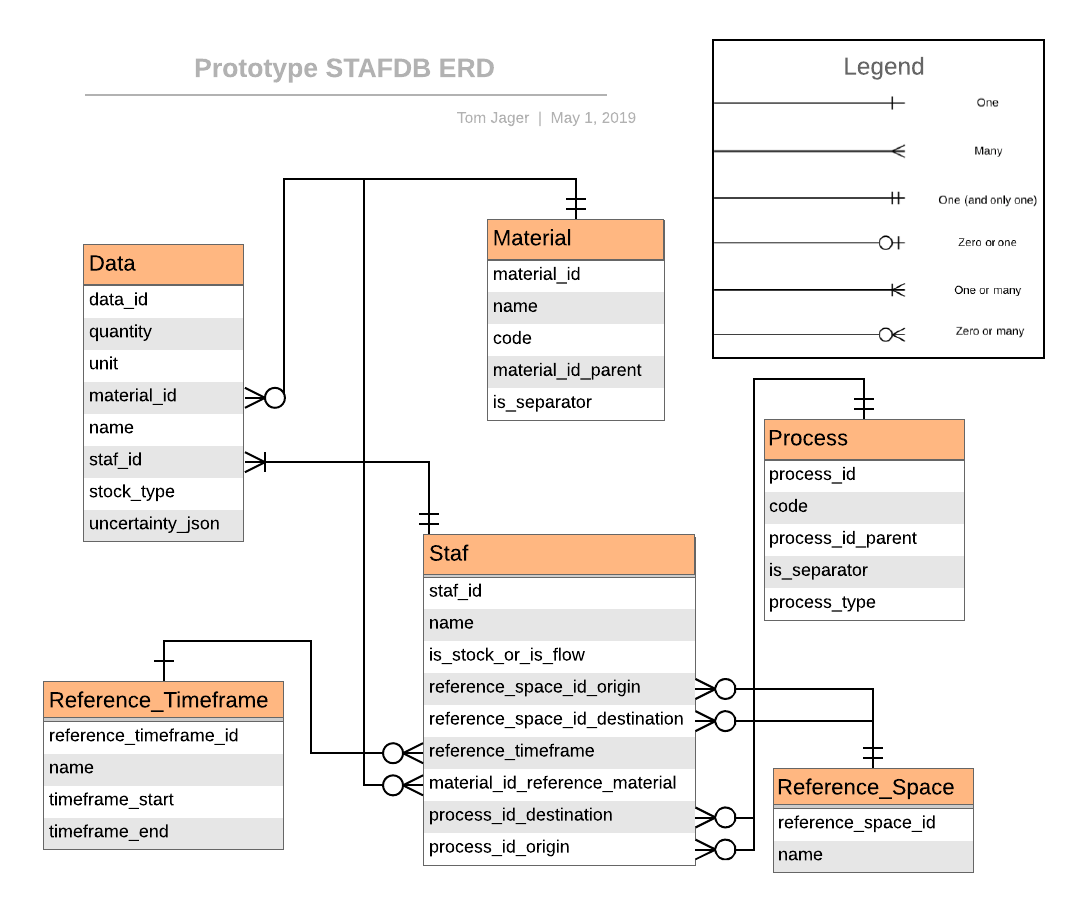
\includegraphics{images/Prototype_STAFDB_ERD.png}
    \caption{Entity Relationship Diagram showing the schema of STAFDB-P}
    \label{fig:prototype_ern}
\end{figure}

STAFDB is designed around describing all industrial ecology systems in terms of stocks and flows which are consolidated into a single entity, STAF. STAFs have associated attributes describing the space, material, timeframe and processes they are in reference to. A STAF is associated with at least one data value. The data value contains information regarding the quantity, unit and specific material that is flowing or being stored. STAFs are associated with multiple data values when they are describing a composite material; each data value is used to describe a fundamental component of the composite material. STAFDB also stores information regarding the provenance of the data, such as the data's quality and the study it has originated from. In \cite{laner2014systematic}, Laner describes a method for expressing a data's quality as uncertainty in the form of normal and log-normal distributions, however no definitive method has been proposed yet for STAFDB. Therefore I have replaced information regarding the provenance of the data with JSON strings describing the data's uncertainty. The uncertainty can be characterised as uniform with a lower or upper bound, or as normally or lognormally distributed with a mean and standard deviation.

\subsection{UMIS Diagram}
% A UMIS diagram is constructed from three components, a list of external flows entering the system, a list of stocks and flows internal to the system, and a list of flows exiting the system.
\label{sec:python_umis_diagram}
A UMIS diagram is used to represent the relationship between stocks, flows and processes. STAF records are first extracted by their ID from STAFDB-P and parsed into sets of \texttt{Stock} and \texttt{Flow} python objects as well as their related attributes. Stocks and flows are separated from STAFs in a UMIS diagram as they have differing behaviour. Both \texttt{Stocks} and \texttt{Flows} inherit from a \texttt{Staf} class which has attributes for time frame, material, origin process and destination process. Stock and flow also have a dictionary which maps a material to its \texttt{StockValue} and \texttt{Value} respectively. These values are the information regarding the quantity of that material being stored or flowing. Both \texttt{StockValue} and \texttt{Value} store the quantity, unit and uncertainty around the data. The uncertainty is simply the serialized JSON string described in section \ref{sec:prototype_stafdb}. \texttt{StockValue} contains an additional field describing the "stock type". This is because stocks in STAFDB may refer to the total amount stored at that process or instead the net transfer of material to or from storage during this time frame.
%If you want to pad stuff out, just have a table showing the representation of JSON strings to their meaning
Origin and destination processes for stocks and flows are parsed into \texttt{UmisProcess} objects. In STAFDB, processes are generalised so that one process record can be used to describe the same event in various locations. For example a manufacturing process in STAFDB can be used to represent manufacturing in Spain or the UK or the USA. In a UMIS diagram, processes must be differentiated by location (space) as flows between the same processes but in different reference spaces are supported. Therefore \texttt{UmisProcess}'s have a unique diagram ID formed of concatenating their process ID and their reference space ID. Processes also store information about their type and name. When a flow is parsed, its origin and destination process is validated to ensure that they are between a transformation and distribution process. Likewise, stocks are validated to ensure that they are between a storage and a transformation or distribution process.

UMIS diagrams are implemented as the class \texttt{UmisDiagram}. They are constructed from sets of external flows entering the diagram, internal stocks and flows in the diagram, and flows exiting the diagram. In agreement with the findings of Myers and Pauliuk \cite{myers2019unified, pauliuk2015general}, the diagram follows a graph pattern \cite{klein}. Therefore, external inflows and external outflows to the system are stored as separate sets, whilst the internal flows and stocks in the diagram are stored as a dictionary mapping each internal process to its outflows and its stock if it has one. The intention is to develop a python representation of a UMIS diagram that is decoupled both from STAFDB and from the Bayesian inference engine. Therefore if further computational models or visualisation tools are developed, they can build directly off of the python classes, without having to write new methods for extracting the data from STAFDB. A UML diagram of the structure of \texttt{UmisDiagram} and its components can be seen in figure \ref{fig:UmisDiagram}.

\begin{figure}
    \centering
    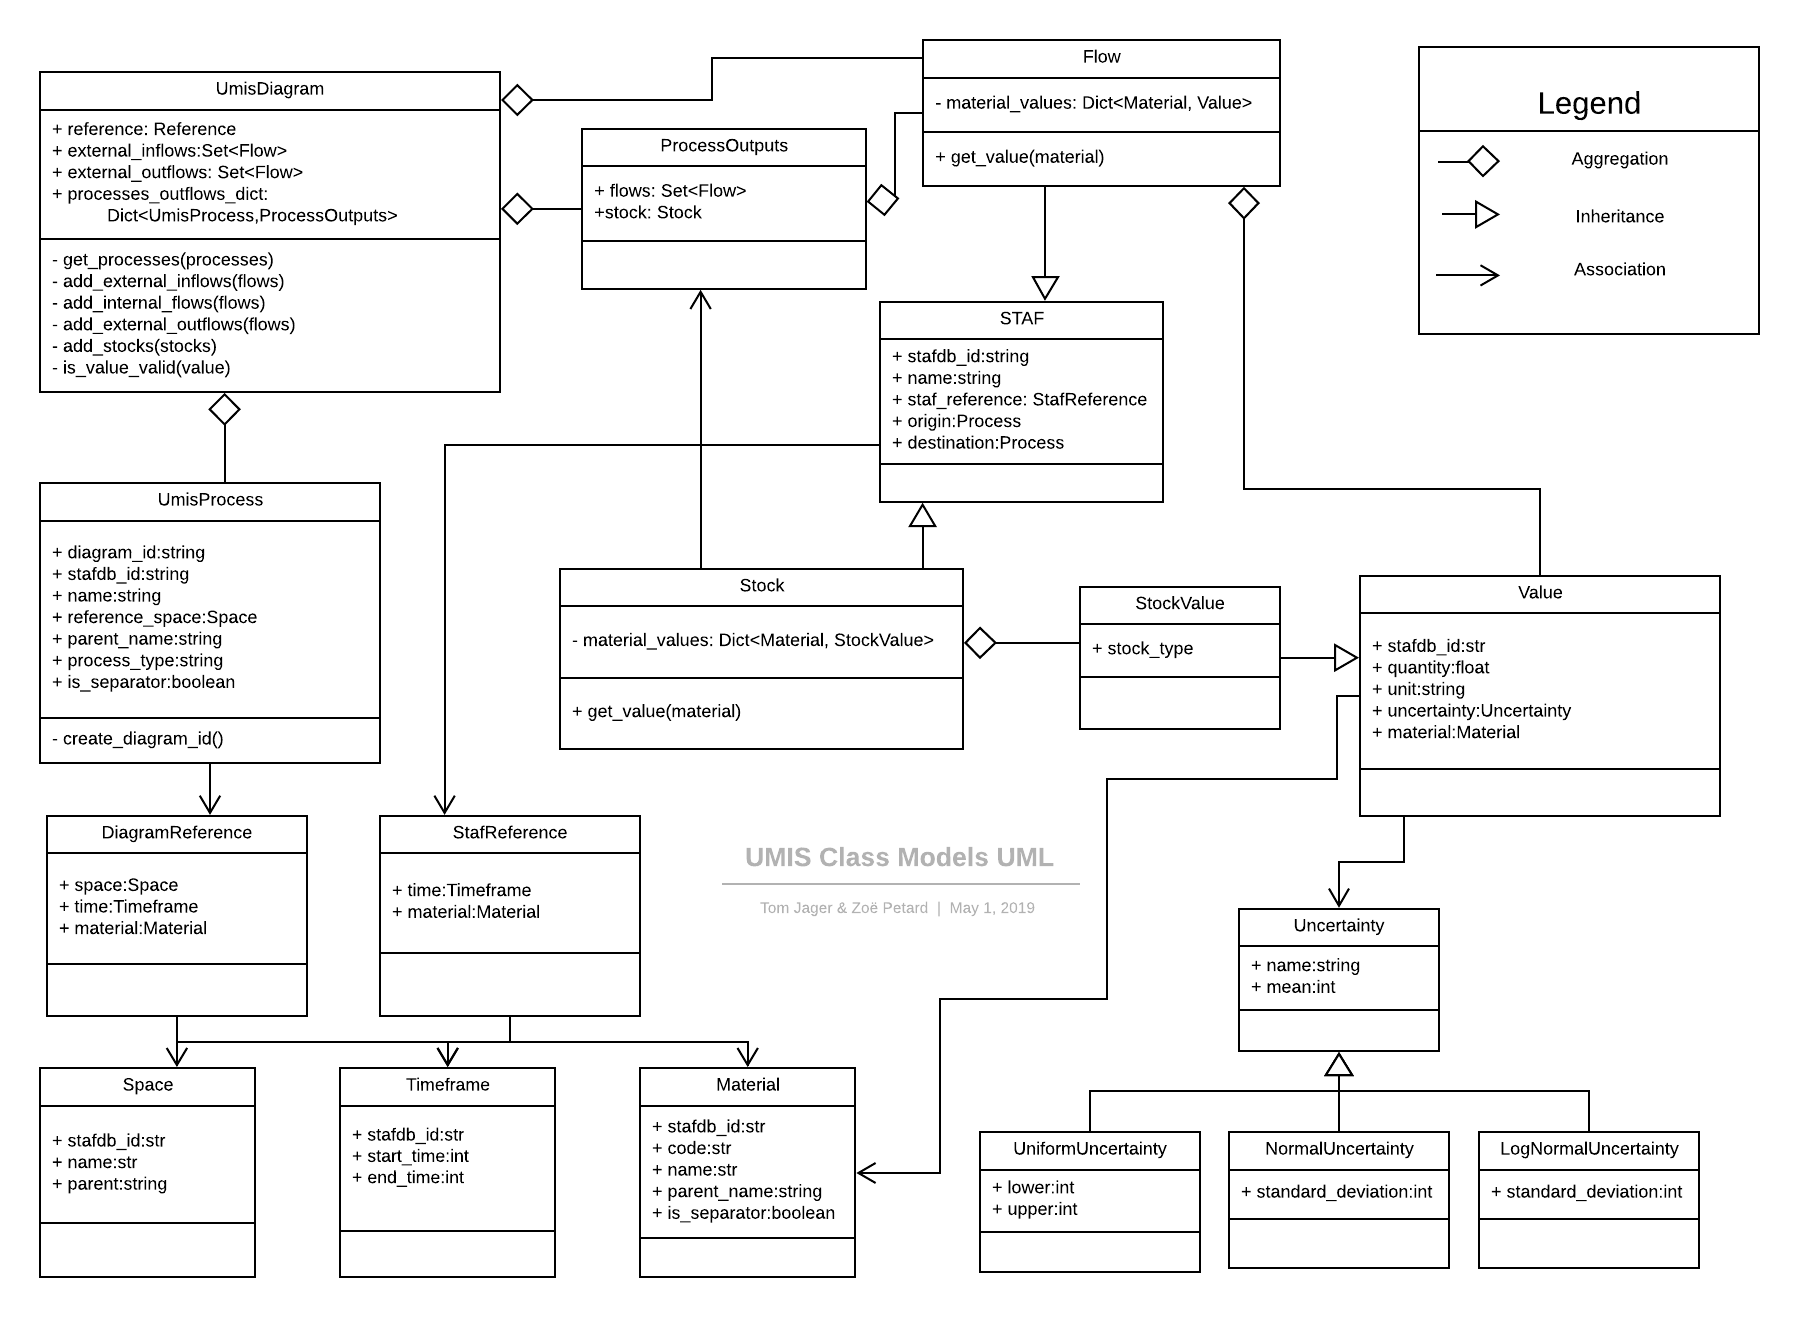
\includegraphics[width=\textwidth]{images/UMIS-data-models.png}
    \caption{UML Class diagram of UMIS diagram data models}
    \label{fig:UmisDiagram}
\end{figure}

Now that stocks and flows have been organised into a UMIS diagram, they can be used to construct a mathematical model, whose parameters can then be inferred with accurate, calibrated uncertainty using Bayesian inference.

\section{Constructing the Mathematical Model}
\subsection{A System of Equations}
In \cite{lupton2018incremental, gottschalk2010probabilistic}, Lupton and Gottschalk use the following equation to model the mass balance constraints of the system:

\begin{equation}
    (I - A)\bullet\bm{z} = \bm(q)
\end{equation}

where $I$ is the identity matrix, $A$ is a matrix of transfer coefficients (TCs) and $a_{ij} \in A$ is the TC from equation \ref{eq:mass_balance_3}, representing the proportion of throughput from process $i$ that moves to process $j$. $\bm{z}$ is a vector of process throughputs as mentioned in equation \ref{eq:mass_balance_2}, $\bm{q}$ is a vector of external inflows to each process from outside the system, and $\bullet$ is the dot product operation.

From equation \ref{eq:mass_balance_3}, we know:

\begin{equation}
    F=A \cdot \bm{z}
\end{equation}

where $f_{ij} \in F$ is the flow from process $i$ to process $j$ and $\cdot$ is the elementwise multiplication operation. Therefore equations for each outflow from processes in Lupton and Gottschalk's models can be derived as:

\begin{equation}
    F=A \cdot (I-A)^{-1} \bullet \bm{q}
\end{equation}

In the context of Cencic's framework, $A$ and $\bm{q}$ can be seen as free observed parameters. Matrix $F$ can be seen as a matrix of dependent observed parameters constructed from free parameters. 

% with a known prior distribution ($p(A)$, $p(\bm{q})$). This prior distribution does not need to be specific, for example the knowledge that all TCs must be between 0 and 1 and that the sum of all outgoing TCs for a process must equal 1 is often sufficient and can be applied to all TCs.
% There is a known prior distribution of these values ($(p(F)$) which is independent from the prior distribution of the free parameters. These prior distributions can take the form of 

Whilst this equation was sufficient for Lupton and Gottschalk's case studies, UMIS systems can include the use of stocks where material flow in and out of a virtual reservoir. Furthermore, UMIS systems can allow for the storage and flow of composite materials. Therefore, concentration coefficients (as in equation \ref{eq:mass_balance_4}) must be included in order to reconcile the flow of composite materials into a reference material.

To accommodate the introduction of stocks, stock values can be separated into two types. In the first, material is stored into the virtual reservoir ($\bm{s^-})$. These are treated as an extra outflow from an existing process into a new storage process. As such they have their own TCs ($A'$) and staf equations ($F' = \begin{bmatrix}
F & \bm{s^-}
\end{bmatrix}$). In the second type, material enters the system from the virtual reservoir ($\bm{s^+}$); these are now treated as another form of inputs to processes in the system ($Q = \begin{bmatrix}\bm{q} & \bm{s^+}
\end{bmatrix}
$).

In order to ensure that the system of equations is mass balancing correctly and that the likelihoods of dependent parameters are being calculated in terms of the same material, concentration coefficients are needed to reconcile staf values for composite materials into the reference material. Input parameters ($Q$) must be converted into the reference material for use in the equations through:

\begin{equation}
    Q_r = Q \cdot {C_{Q}}
\end{equation}

The results from staf equations must also be converted from the reference material into the material that is observed through:
\begin{equation}
    F'_o = \frac{F'}{C_{F'}}
\end{equation}


Therefore the system of equations for my model is:

\begin{equation}
    F'_o = \frac{A' \cdot (I-A)^{-1} \bullet sum(Q \cdot C_Q)}{C_{F'}}
    \label{eq:my_model_eq}
\end{equation}

where $F'_o$ are dependent observed parameters whilst $A', Q, C_Q$ and $C_{F'}$ are free observed parameters.
\subsection{Representing Model Parameters}
Each parameter in the model has a known prior distribution $p(x)$ which characterises the uncertainty around that parameter's true value. For $Q$, $F'_o$, $C_{Q}$ and $C_{F'}$ these can be represented as normally, log-normally or uniformly distributed stochastic variables whose distribution parameters are $\{\mu_n, \sigma_n\}$, $\{\mu_l, \sigma_l\}$ and $\{l_u, u_u\}$ respectively. The values for $F'_r$ and $Q$ are supplied when constructing the UMIS diagram and take the form of \texttt{Uncertainty} attributes in the corresponding \texttt{Stock} and \texttt{Flow} objects. A material reconciliation table is supplied to the system and is used to map materials to the prior distributions of CCs.

\subsubsection{Representing TCs}
\label{sec:representing_tcs}
TCs have a more interesting prior distribution as their value relies on the structure of the model and differ according to their process type. Lupton also recognises the division of transformation and distribution processes and proposes characterising the TCs of each process type through different distributions. For both types if a process only has one outflow then its TC must be 1, whilst if there are no outflows, the TC must be 0. The modeller may have prior knowledge of TC values that they wish to supply to the model. This can be done through the use of a TC lookup table which maps the origin process and destination process IDs of the TC to an \texttt{Uncertainty} object. 

Transformation processes can have at most 2 outflows: a stock and an outflow to another process. In this case, the TCs must be $a$ and $1-a$. If no prior knowledge of the TC exists, then $a$ is represented as a uniform distribution between 0 and 1. If prior knowledge about one TC exists in the lookup table, $a$ is represented as the stochastic variable from that \texttt{Uncertainty}. If prior knowledge about both exists, then one is arbitrarily selected to model $a$.

Distribution processes can have many outflows, including to stock. Lupton models these TCs as parameters from a Dirichlet distribution. A Dirichlet distribution is a continuous multivariate distribution with two parameters $\bm{\alpha}$ and $\bm{\theta}$ \cite{dirichlet}. Drawing from a Dirichlet distribution results in $\{theta_1, ..., \theta_n\} = \bm{\theta}$ where $\sum_{i}\theta_i = 1$ and $\theta_i \ge 0$. This makes it ideal for representing TCs. The share parameters $\{\alpha_1, ..., \alpha_n\} = \bm{\alpha}$ indicate a weighting to a certain configuration of $\bm{\theta}$. Figure \ref{fig:dirichlet} shows the effect of $\bm{\alpha}$ on a three parameter Dirichlet distribution. If no prior knowledge of TCs exist, each $\alpha_i$ is set to 1 resulting in every possible configuration of TCs being equally likely. If prior knowledge of any TC exists in the lookup table, its $\alpha$ is set to the mean of the \texttt{Uncertainty} object.

\begin{figure}
    \centering
    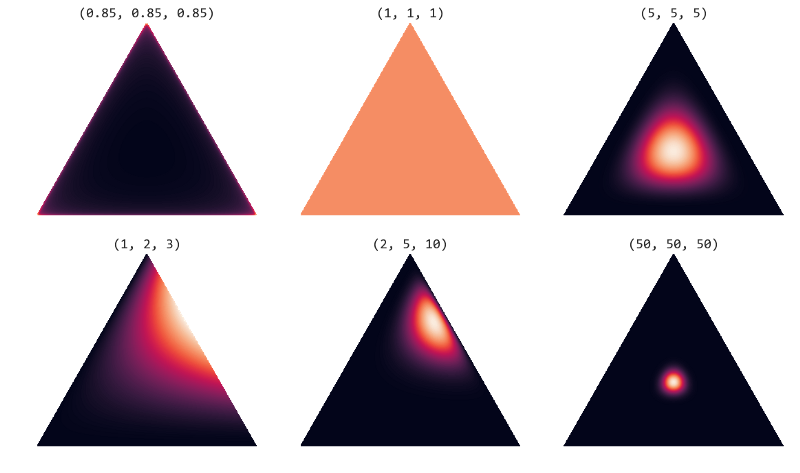
\includegraphics[width=0.75\textwidth]{images/dirichlet.png}
    \caption{Effect of $\bm{\alpha}$ on a three parameter Dirichlet distribution. Source: \cite{dirichlet}}
    \label{fig:dirichlet}
\end{figure}

\subsection{Model Construction}
In his implementation, Lupton used Pymc3 to create his mathematical model from stochastic variables, observe the likelihood of his dependent parameters and sample from the resultant posterior distribution. He used Theano operations to define the equations in his system. We will use the same tools in our approach. Construction of the model before sampling can be split into three stages: Defining the parameter priors, creating the model parameters and equations, and observing the dependent parameters to calculate their likelihood. This structure is illustrated in figure \ref{fig:inference_engine_structure}.

\newgeometry{left=0cm,bottom=0cm, right=0cm,top=0cm}
\begin{figure}
    \centering
    % 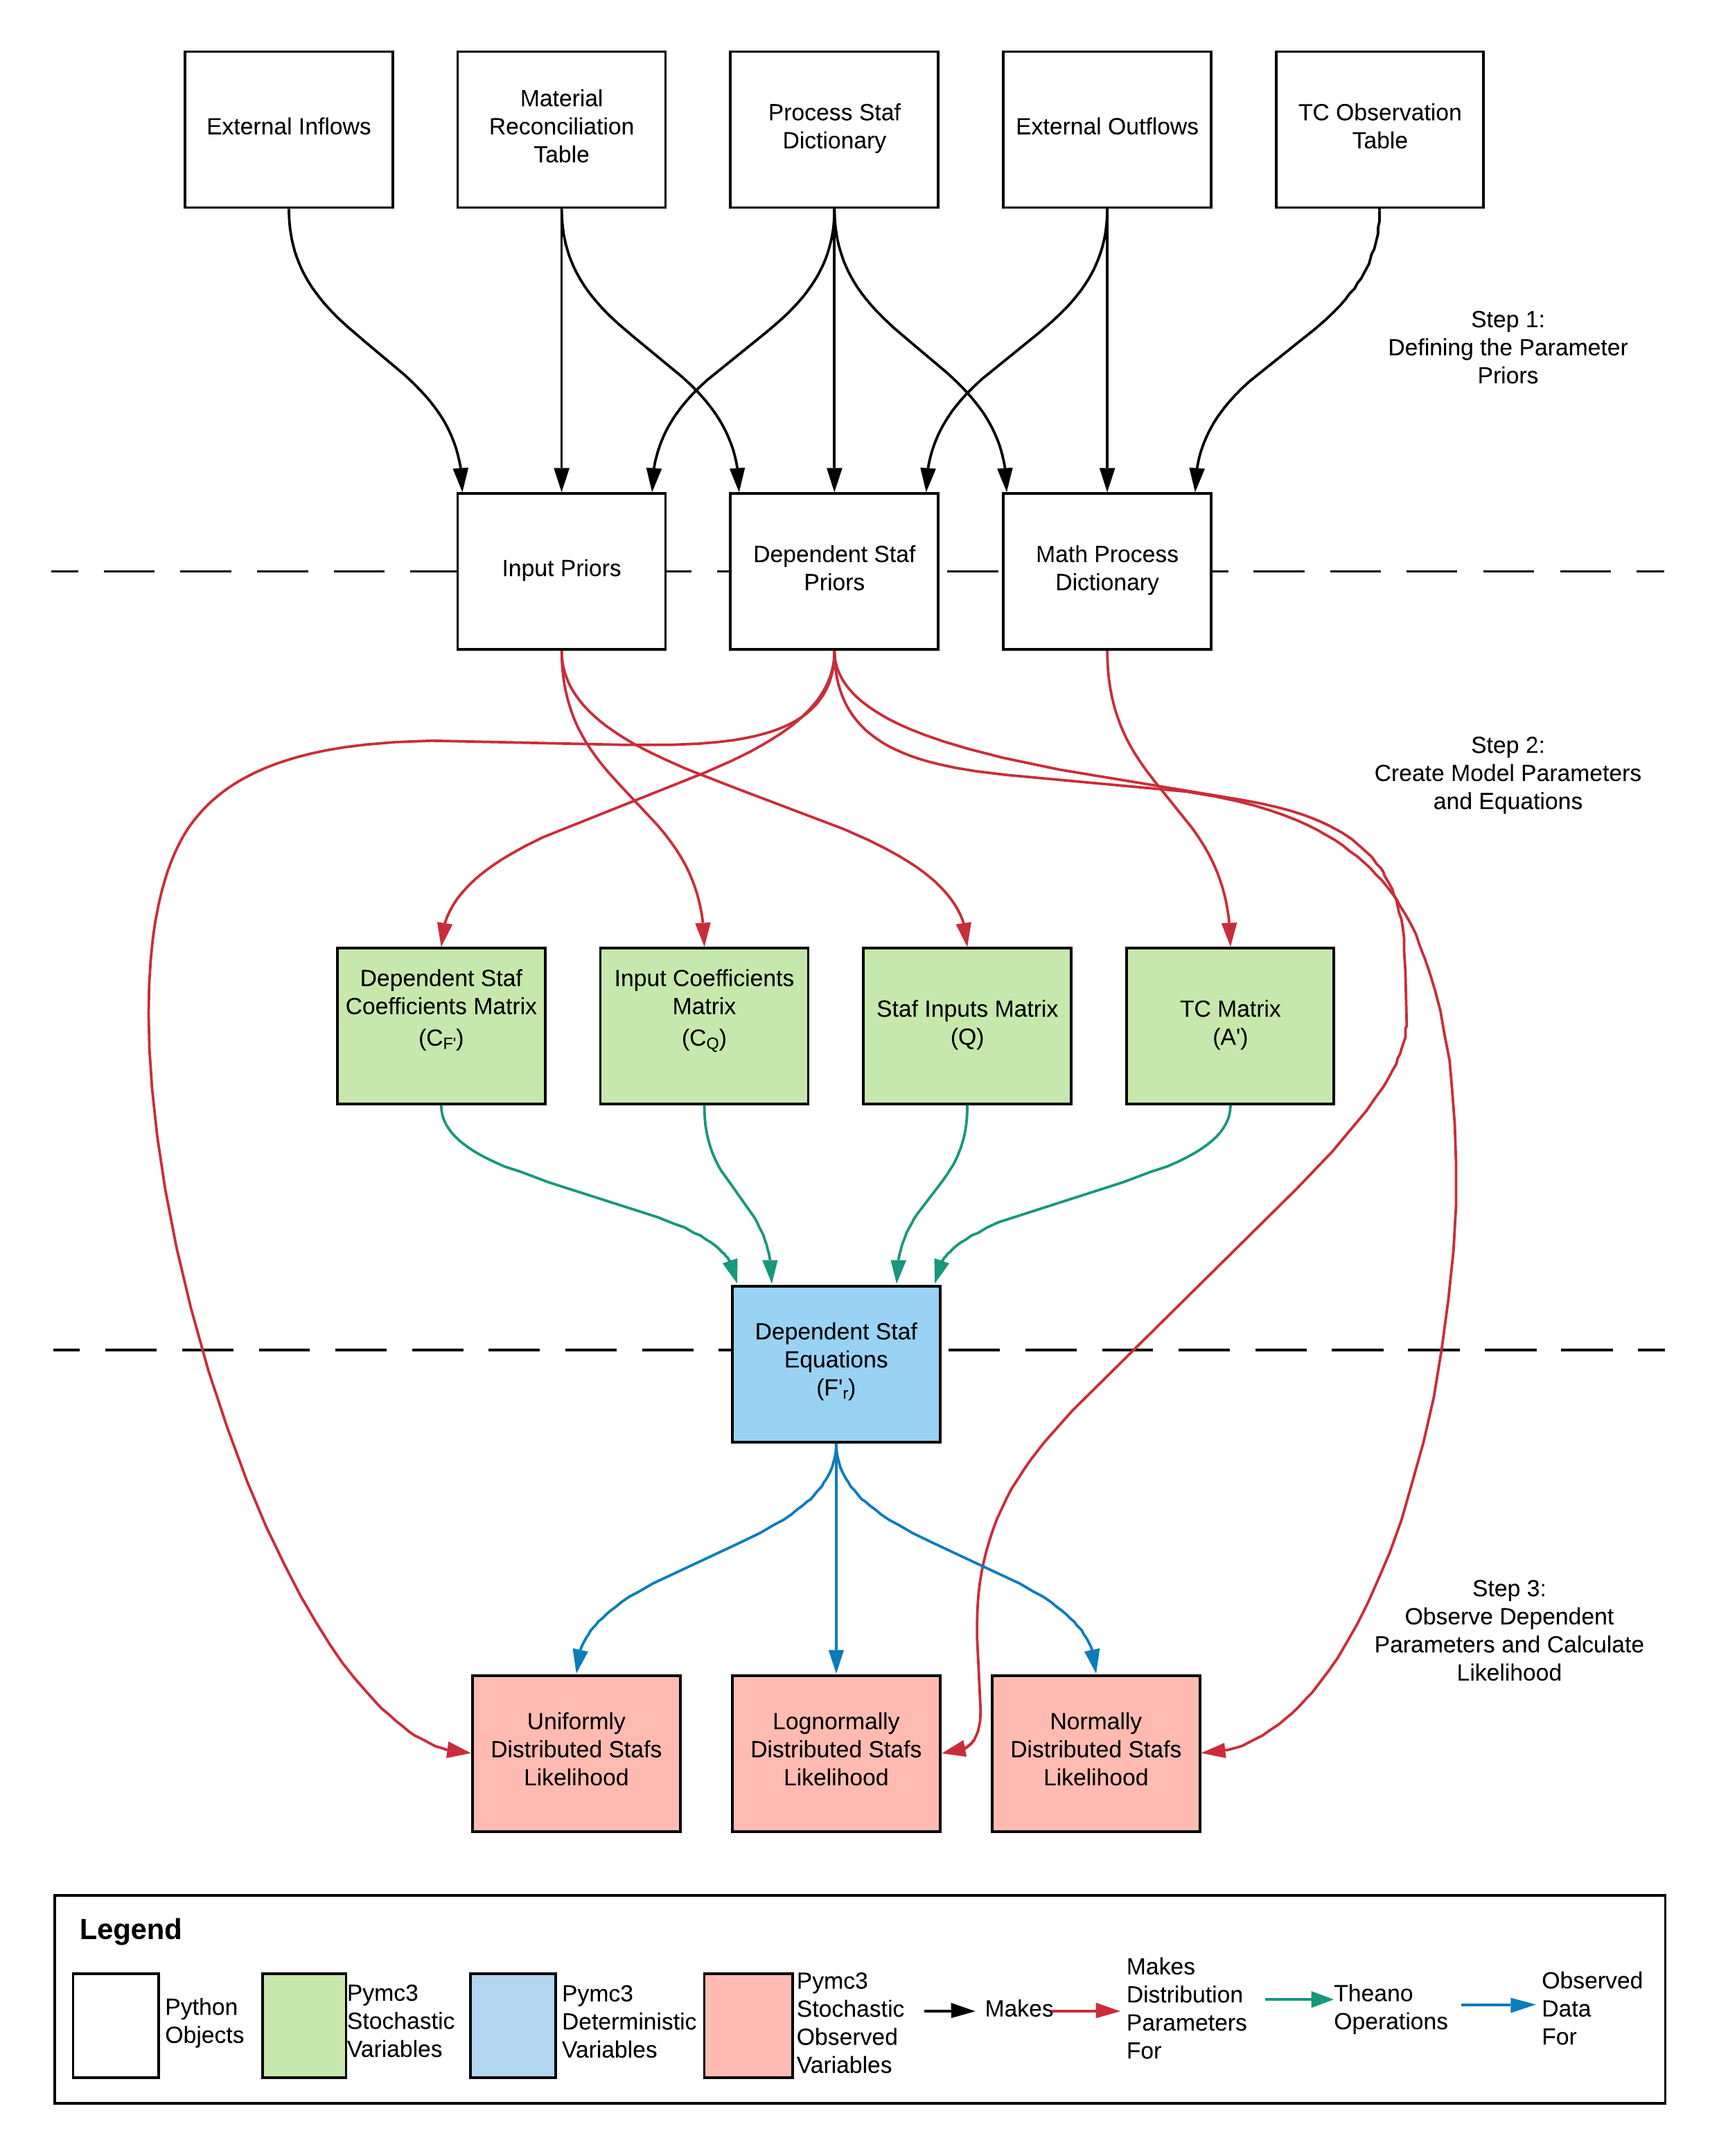
\includegraphics[width=\paperwidth]{images/inference_engine_structure.png}
    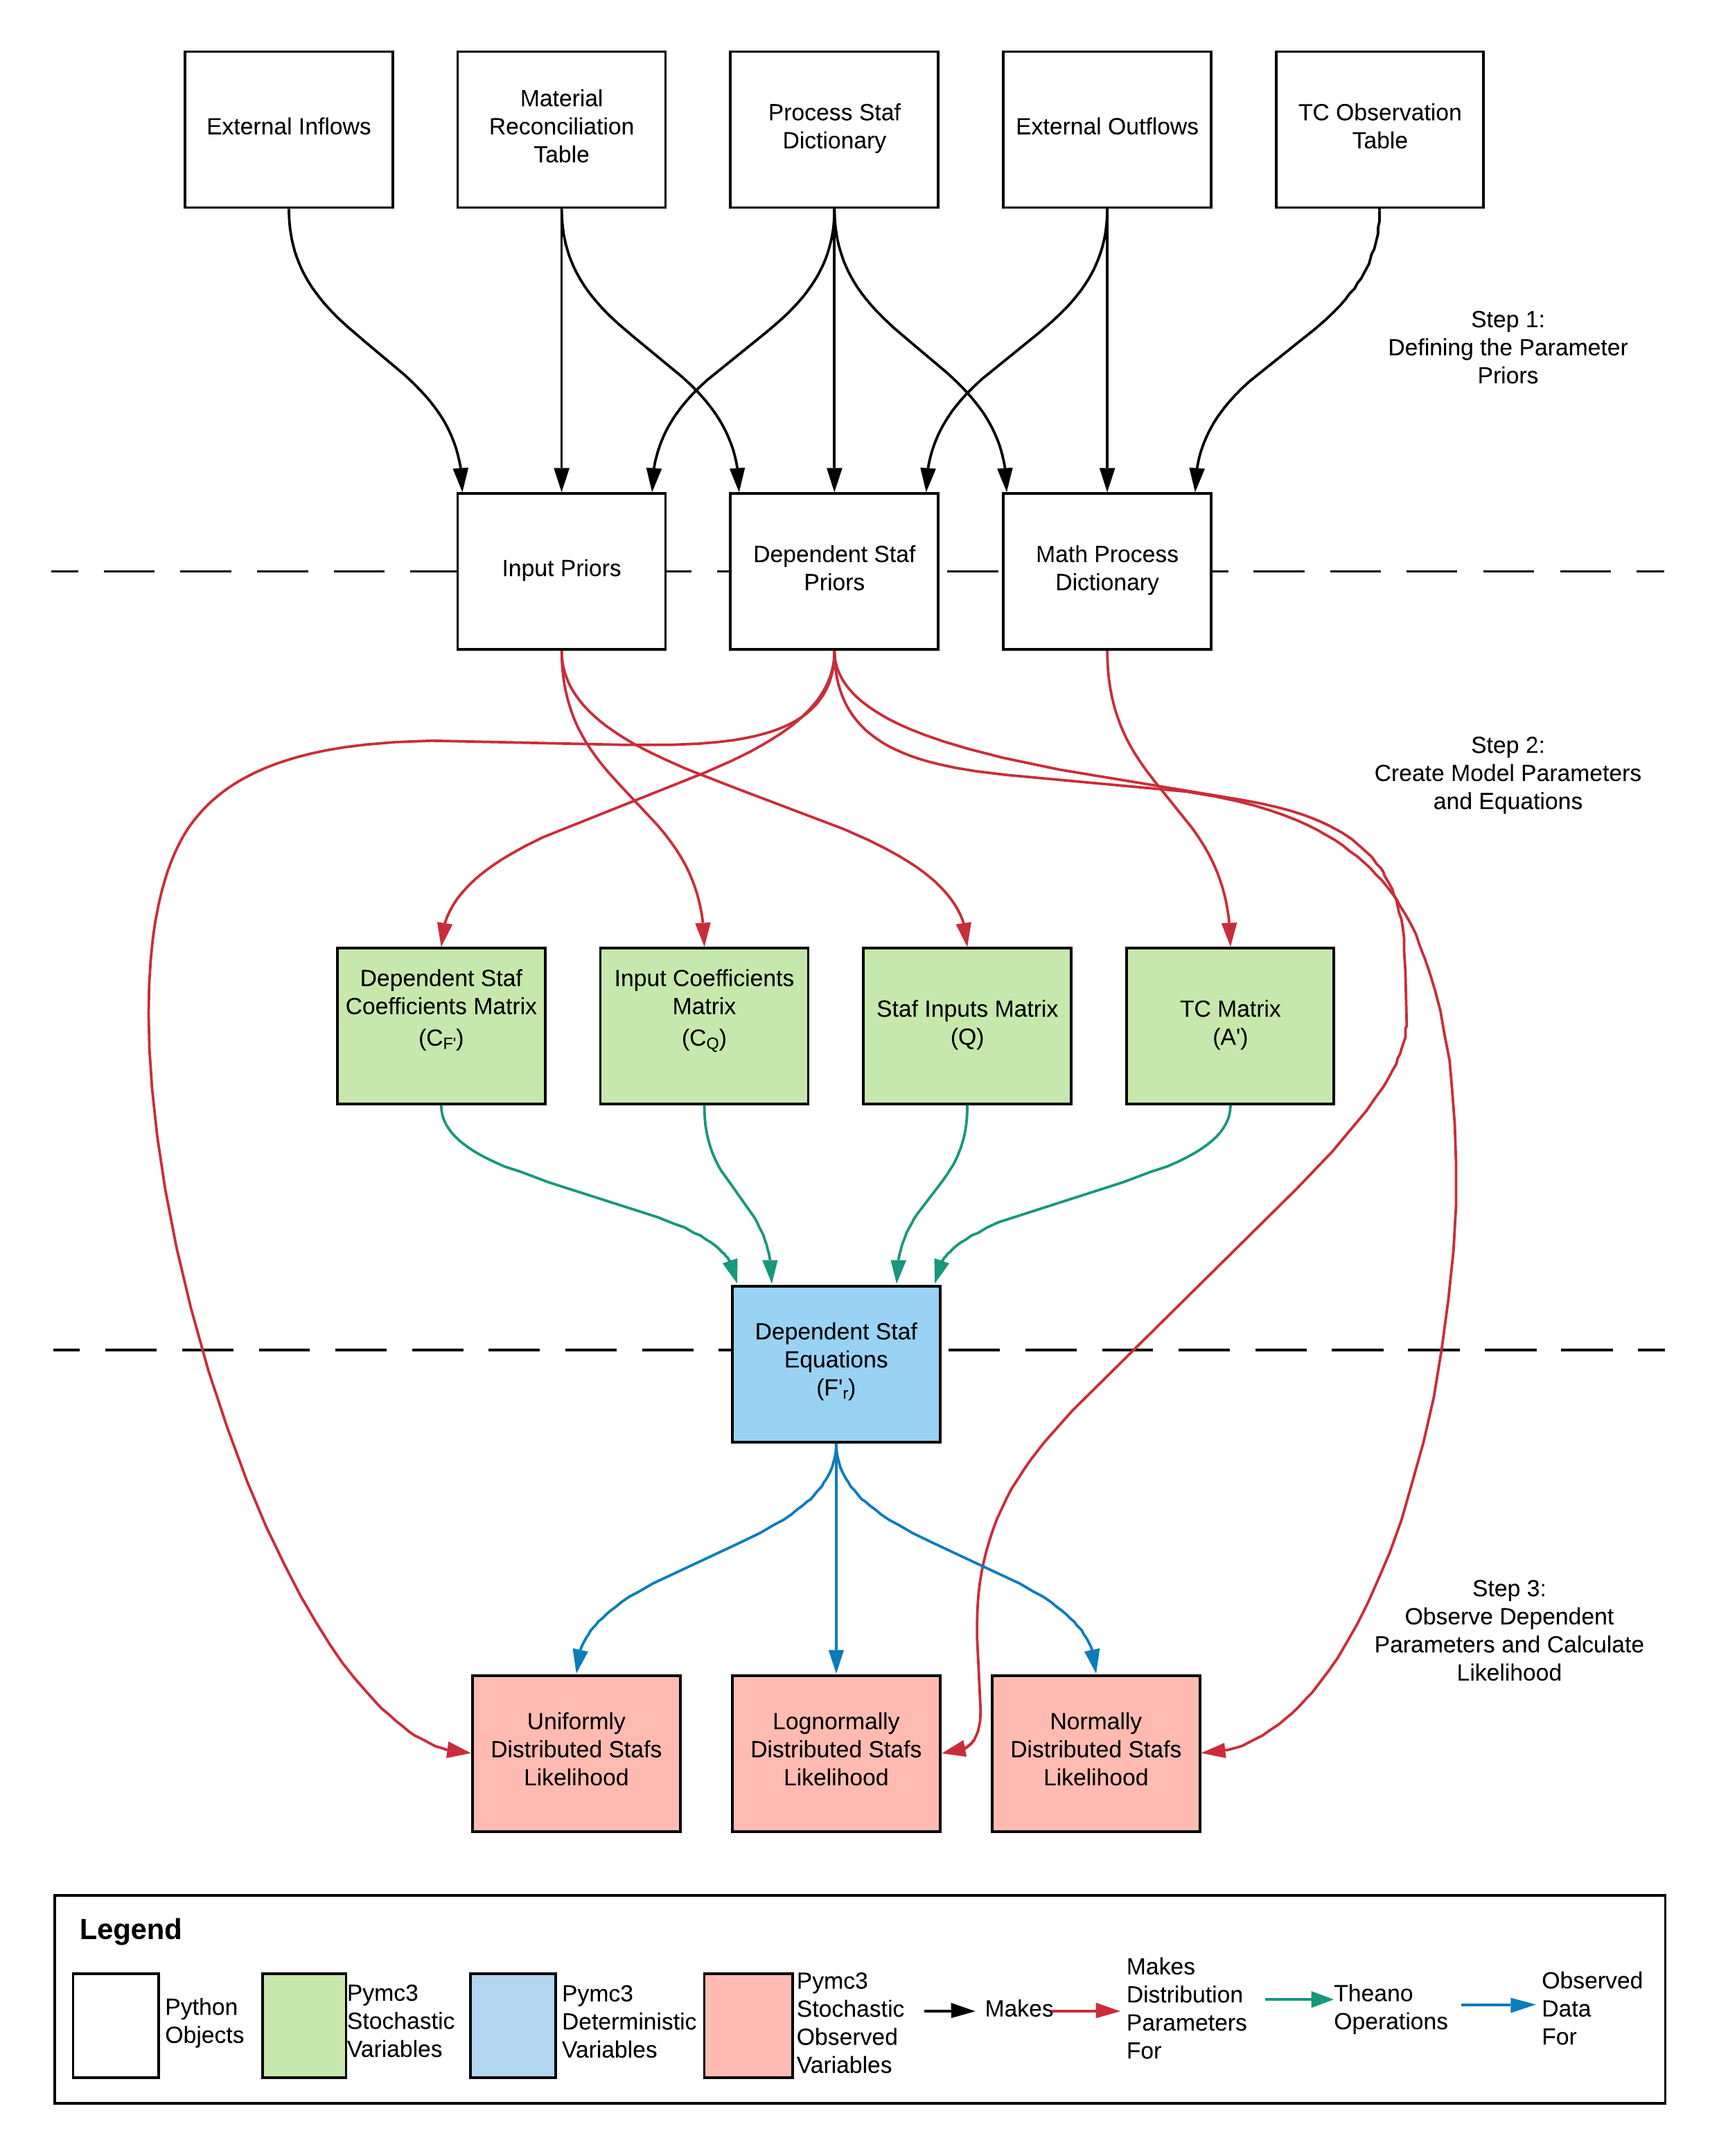
\includegraphics[width=0.9\paperwidth]{images/inference_engine_structure.png}
    \caption{Structure of model construction for the Bayesian inference engine}
    \label{fig:inference_engine_structure}
\end{figure}
\restoregeometry

\subsubsection{Stage 1: Defining Parameter Priors}
The first stage is devoted to creating python objects which are in turn used to create the stochastic random variables which represent parameters in the model. It takes as input the python object representation of the UMIS diagram, a material reconciliation table, a TC observation table and reference attributes. The material reconciliation table maps a material to its concentration coefficient. The reference attributes refer to the specific time frame and material over which the system is mass balanced. On processing stocks and flows, if they belong to the wrong time frame then they are ignored. If the stock or flow does not have a value for the reference material, it undergoes material reconciliation. This checks to see if the stock or flow has a value for a material corresponding to an entry in the material reconciliation table. If so, that value is used and that materials CC is stored for use later. If a stock or flow has no material that can be reconciled, it is ignored. If no material reconciliation is necessary a deterministic CC of 1 is used. The TC observation table is used to store prior information about TC values. Its design and use is discussed in section \ref{sec:representing_tcs}. The python representation of the UMIS diagram consists of the list of External Inflows, dictionary of processes to internal stafs (Internal Stafs Dictionary) and list of External Outflows discussed in section \ref{sec:python_umis_diagram}.

The first python objects constructed are the Math Processes and the Math Process Dictionary. This maps the diagram ID of the process to its corresponding math process. This allows for looking up the Math Processes later which is useful for placing model parameters in the correct positions in parameter matrices. On creation of a new Math Process it is assigned an automatically increasing process index which refers to its row in the parameter matrices. Construction is performed by iterating over the Internal Stafs Dictionary and External Outflows.

Outflows are added to a process as ParamPrior objects. These contain a parameter's type (e.g TC), origin process ID, destination process ID and an uncertainty attribute which describes its distribution. ParamPrior objects have a method to construct a Pymc3 stochastic variable corresponding to the parameter's uncertainty. For these ParamPrior objects, the uncertainty refers to the prior knowledge of the TC for the outflow. Math Processes have a method to use its outflows to create a list of process IDs that receive flows from it, and a corresponding list of stochastic variables representing its TCs. These stochastic variables are constructed in accordance with section \ref{sec:representing_tcs}. Any stocks that are coming from the virtual reservoir ($s^+$) are ignored, whilst stock going to the virtual reservoir ($s^-$) are represented as an outflow to a process has no outflows.

Next the InputPriors object is created. This contains two dictionaries, one mapping process IDs to their inputs from External Inflows (External Inflows Dictionary) and the other mapping process IDs to the inputs from Stock Inputs (Stock Inputs Dictionary). Each input is represented by two ParamPrior objects, one representing the un-reconciled staf value flowing into the system ($\{q_i | s^+_i\} \in Q$) and the other representing its CC ($c_q \in C_q)$. The External Inflows are iterated over to construct the External Inflows Dictionary whilst Stock Inputs Dictionary is constructed from the Internal Stafs Dictionary.

The final python object is the Dependent Staf Priors. This is a list of Dependent Staf Prior objects. Each Dependent Staf Prior consists of two ParamPrior objects, one representing the un-reconciled observed distributions of the dependent model parameters ($f'_o \in F'_o$) and the other representing its CC ($c_r \in C_{F'}$). Dependent Staf Priors separate the observed parameters into three lists by their distributions.

\subsubsection{Stage 2: Create Model Parameters and Equations}
Once the python objects have been created they are used to develop a Pymc3 mathematical model. The matrices in the right hand side of equation \ref{eq:my_model_eq} are constructed as Theano tensors and then populated either by Pymc3 stochastic variables or constants.

First the TC matrix ($A'$) is constructed from the Math Process Dictionary. It is initialised as an $N_p \times N_p$ dimensional Theano matrix of zeros, where $N_p$ is the number of processes in the system (including new ones created from stock values). The Math Process Dictionary is then used to create the Pymc3 stochastic random variables for each TC and place them in the correct positions in the matrix. Similarly, the Staf Inputs Matrix  ($Q$) and its corresponding Input Coefficients Matrix ($C_Q$) are constructed as Theano tensors and populated by stochastic random variables from the Input Priors. By adding these random variables to the Pymc3 model they are set as free variables in a mathematical model. Later when this model is sampled from, proposals will be drawn as a vector of these free variables.

Each Theano matrix as a whole is set as a named Pymc3 deterministic variable. When this model is sampled, Pymc3 will then store the value of each matrix for each sample. This allows us to extract the posterior samples of each matrix from their variable name and then access specific parameters using their location in that matrix. 

%TODO make a table mapping the python object names in the diss to their names in the implementation and put it in the appendix
%Dependent Staf Priors, Dependent Staf Prior, External Inflows Dictionary, Internal Stafs Dictionary, Math Process, Math Processes Dictionary,  Stock Inputs Dictionary

%TODO Talk about pymc3, allows for the creation of mathematical models. Can create free variables, define deterministic variables as theano operations of the free variables, include likelihood terms as the likelihood of observing values given a distribution
% Can say we did validation but probs don't need to
% Maybe get rid of the last sentence
\begin{comment}
 {\bf A topic-specific chapter, of roughly $15$ pages} 
\vspace{1cm} 

% Maybe explain what aggregation, association and inheritance are
% Maybe say that disaggregation stuff, processes and materials contain fields to talk about disaggregation so no double counting, not implemented here
\noindent
This chapter is intended to describe what you did: the goal is to explain
the main activity or activities, of any type, which constituted your work 
during the project.  The content is highly topic-specific, but for many 
projects it will make sense to split the chapter into two sections: one 
will discuss the design of something (e.g., some hardware or software, or 
an algorithm, or experiment), including any rationale or decisions made, 
and the other will discuss how this design was realised via some form of 
implementation.  

\noindent
Note that it is common to include evidence of ``best practice'' project 
management (e.g., use of version control, choice of programming language 
and so on).  Rather than simply a rote list, make sure any such content 
is useful and/or informative in some way: for example, if there was a 
decision to be made then explain the trade-offs and implications 
involved.

\end{comment}

\begin{comment}
 - For execution, a low level of sample acceptance is indicative of a mistake when describing the system, therefore the system must be re-described
  - Execution, umis as classes (decisions)
\end{comment}

% -----------------------------------------------------------------------------

\chapter{Critical Evaluation}
\label{chap:evaluation}


\begin{comment}
{\bf A topic-specific chapter, of roughly $15$ pages} 
\vspace{1cm} 

\noindent
This chapter is intended to evaluate what you did.  The content is highly 
topic-specific, but for many projects will have flavours of the following:

\begin{enumerate}
\item functional  testing, including analysis and explanation of failure 
      cases,
\item behavioural testing, often including analysis of any results that 
      draw some form of conclusion wrt. the aims and objectives,
      and
\item evaluation of options and decisions within the project, and/or a
      comparison with alternatives.
\end{enumerate}

\noindent
This chapter often acts to differentiate project quality: even if the work
completed is of a high technical quality, critical yet objective evaluation 
and comparison of the outcomes is crucial.  In essence, the reader wants to
learn something, so the worst examples amount to simple statements of fact 
(e.g., ``graph X shows the result is Y''); the best examples are analytical 
and exploratory (e.g., ``graph X shows the result is Y, which means Z; this 
contradicts [1], which may be because I use a different assumption'').  As 
such, both positive {\em and} negative outcomes are valid {\em if} presented 
in a suitable manner.
 
 - Evaluation - turn graedal diagram into UMIS diagram
  - Evaluation - Lognormal, does that work
\end{comment}

% -----------------------------------------------------------------------------

\chapter{Conclusion}
\label{chap:conclusion}

\begin{comment}
{\bf A compulsory chapter,     of roughly $5$ pages} 
\vspace{1cm} 

\noindent
The concluding chapter of a dissertation is often underutilised because it 
is too often left too close to the deadline: it is important to allocation
enough attention.  Ideally, the chapter will consist of three parts:

\begin{enumerate}
\item (Re)summarise the main contributions and achievements, in essence
      summing up the content.
\item Clearly state the current project status (e.g., ``X is working, Y 
      is not'') and evaluate what has been achieved with respect to the 
      initial aims and objectives (e.g., ``I completed aim X outlined 
      previously, the evidence for this is within Chapter Y'').  There 
      is no problem including aims which were not completed, but it is 
      important to evaluate and/or justify why this is the case.
\item Outline any open problems or future plans.  Rather than treat this
      only as an exercise in what you {\em could} have done given more 
      time, try to focus on any unexplored options or interesting outcomes
      (e.g., ``my experiment for X gave counter-intuitive results, this 
      could be because Y and would form an interesting area for further 
      study'' or ``users found feature Z of my software difficult to use,
      which is obvious in hindsight but not during at design stage; to 
      resolve this, I could clearly apply the technique of Smith [7]'').
\end{enumerate}

\end{comment}

% =============================================================================

% Finally, after the main matter, the back matter is specified.  This is
% typically populated with just the bibliography.  LaTeX deals with these
% in one of two ways, namely
%
% - inline, which roughly means the author specifies entries using the 
%   \bibitem macro and typesets them manually, or
% - using BiBTeX, which means entries are contained in a separate file
%   (which is essentially a databased) then inported; this is the 
%   approach used below, with the databased being dissertation.bib.
%
% Either way, the each entry has a key (or identifier) which can be used
% in the main matter to cite it, e.g., \cite{X}, \cite[Chapter 2}{Y}.

\backmatter

\bibliography{dissertation}

% -----------------------------------------------------------------------------

% The dissertation concludes with a set of (optional) appendicies; these are 
% the same as chapters in a sense, but once signaled as being appendicies via
% the associated macro, LaTeX manages them appropriatly.

\appendix

\chapter{Appendix A}
\label{appx:example}

\section{STAFDB Entity Relationship Diagram}
\begin{comment}
Content which is not central to, but may enhance the dissertation can be 
included in one or more appendices; examples include, but are not limited
to

\begin{itemize}
\item lengthy mathematical proofs, numerical or graphical results which 
      are summarised in the main body,
\item sample or example calculations, 
      and
\item results of user studies or questionnaires.
\end{itemize}

\noindent
Note that in line with most research conferences, the marking panel is not
obliged to read such appendices.

\end{comment}

% =============================================================================

\end{document}
